\documentclass{beamer}
\usetheme{Warsaw} % Ou remplacez par votre thème préféré
\setbeamertemplate{headline}{}
\usepackage{amsmath, amsfonts, mathtools}
\usepackage{stmaryrd}
\usepackage{graphicx}
\usepackage{subcaption}
\usepackage{float}
\usepackage{tikz}
\usepackage{pgfplots}
\usepackage{bbold}
\usepackage{bm}  
\usepackage{bbm}
\usepackage{etoolbox}
\usepackage{array}
\usepackage{adjustbox}
\usepackage{caption}

\captionsetup{justification=centering}
\pgfplotsset{compat=1.18} % Version pour PGFPlots
\makeatletter
\patchcmd{\beamer@calculateheadfoot}{\insertcontinuationcount}{\relax}{}{}
\makeatother
\setbeamertemplate{caption}[numbered]

\setbeamertemplate{section page}{
    \begin{centering}
        \begin{beamercolorbox}[sep=12pt,center, rounded = true]{part title}
            \usebeamerfont{section title}\insertsection\par
        \end{beamercolorbox}
    \end{centering}
}


\title{Tensor multiblock logistic regression}
\author{SELVESTREL Alexandre}
\institute{
    Université Paris-Saclay, CNRS, CentraleSupélec, Laboratoire des signaux et systèmes\\[10 pt]
    \textbf{Supervisors :} Arthur Tenenhaus, Laurent Lebrusquet\\[10 pt]
    \textbf{Medical partner :} Henri Mondor hospital, radiologist: Sébastien Mulé
}
\date{\today}

\begin{document}

\begin{frame}
    \titlepage
\end{frame}

% \begin{frame}
%     \frametitle{Liver tumors classification}
%     \begin{center}
%         \textbf{$\mathbf{6}^{\text{th}}$ most widespread cancer and $\mathbf{4}^{\text{th}}$ mortality cause by cancer}\\
%     \end{center}
%     Classification:
%     \begin{itemize}
%         \item Hepatocellular Carcinoma (HCC): $75\%$ of cases, resection often possible\\[10 pt]
%         \item CCK = Cholangiocarcinoma (CCK): $6\%$ of cases, resection difficult (possible in $30\%$ of cases)\\[10 pt]
%         \item Others: benign ($18 \%$ of cases) or Hepatoblastoma ($1 \%$ of cases)
%     \end{itemize}
% \end{frame}

% \begin{frame}
%     \frametitle{Difficulties for classification}
%     \begin{itemize}
%     \item No perfect method using MRI images (contrast, shape, size, location): disagreement between radiologists \\[15 pt]
%     \item High levels of alpha-fetoprotein indicate HCC, but not always.\\[15 pt]
%     \item Biopsy: invasive and potentially lethal ($0.02 \%$ of patients)\\
%     \end{itemize}
%     \begin{center}
%         But a lot of clues even without biopsy $\rightarrow$ Machine Learning
%     \end{center}
% \end{frame}

% \begin{frame}
%     \frametitle{Available data}

%     $\bullet$ MRI images in 3D of liver tumors (arterial, portal, late)\\[5 pt]
%     $\bullet$ gender (63 men, 27 women)\\[5 pt]
%     $\bullet$ age at disease (average: $63$ years old)\\[15 pt]

%     From Henri Mondor hospital: Sébastien Mulé

%     Same variables extracted from each MRI image at 3 times  $\rightarrow$ specific structure\\[10 pt]

%     Need to adapt existing machine learning methods to this structure

    
% \end{frame}


% \begin{frame}
%     \begin{figure}
%         \centering
%         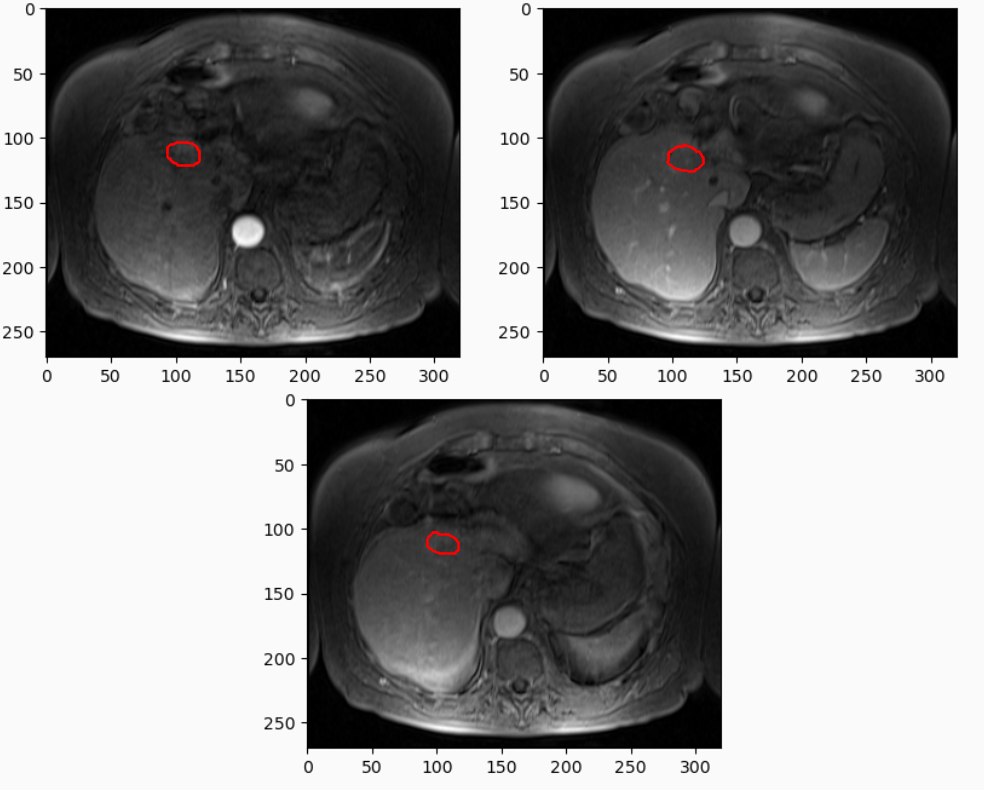
\includegraphics[scale = 0.215]{images/CCK.png}
%         \caption{Example of MRI images of a CCK tumor (arterial, portal, late)}
%     \end{figure}
% \end{frame}


% \begin{frame}
%     \frametitle{Correlation matrix of features about texture (GLDM)}
%     Strong correlations between imaging times for a given variable
%     \begin{figure}
%         \centering
%         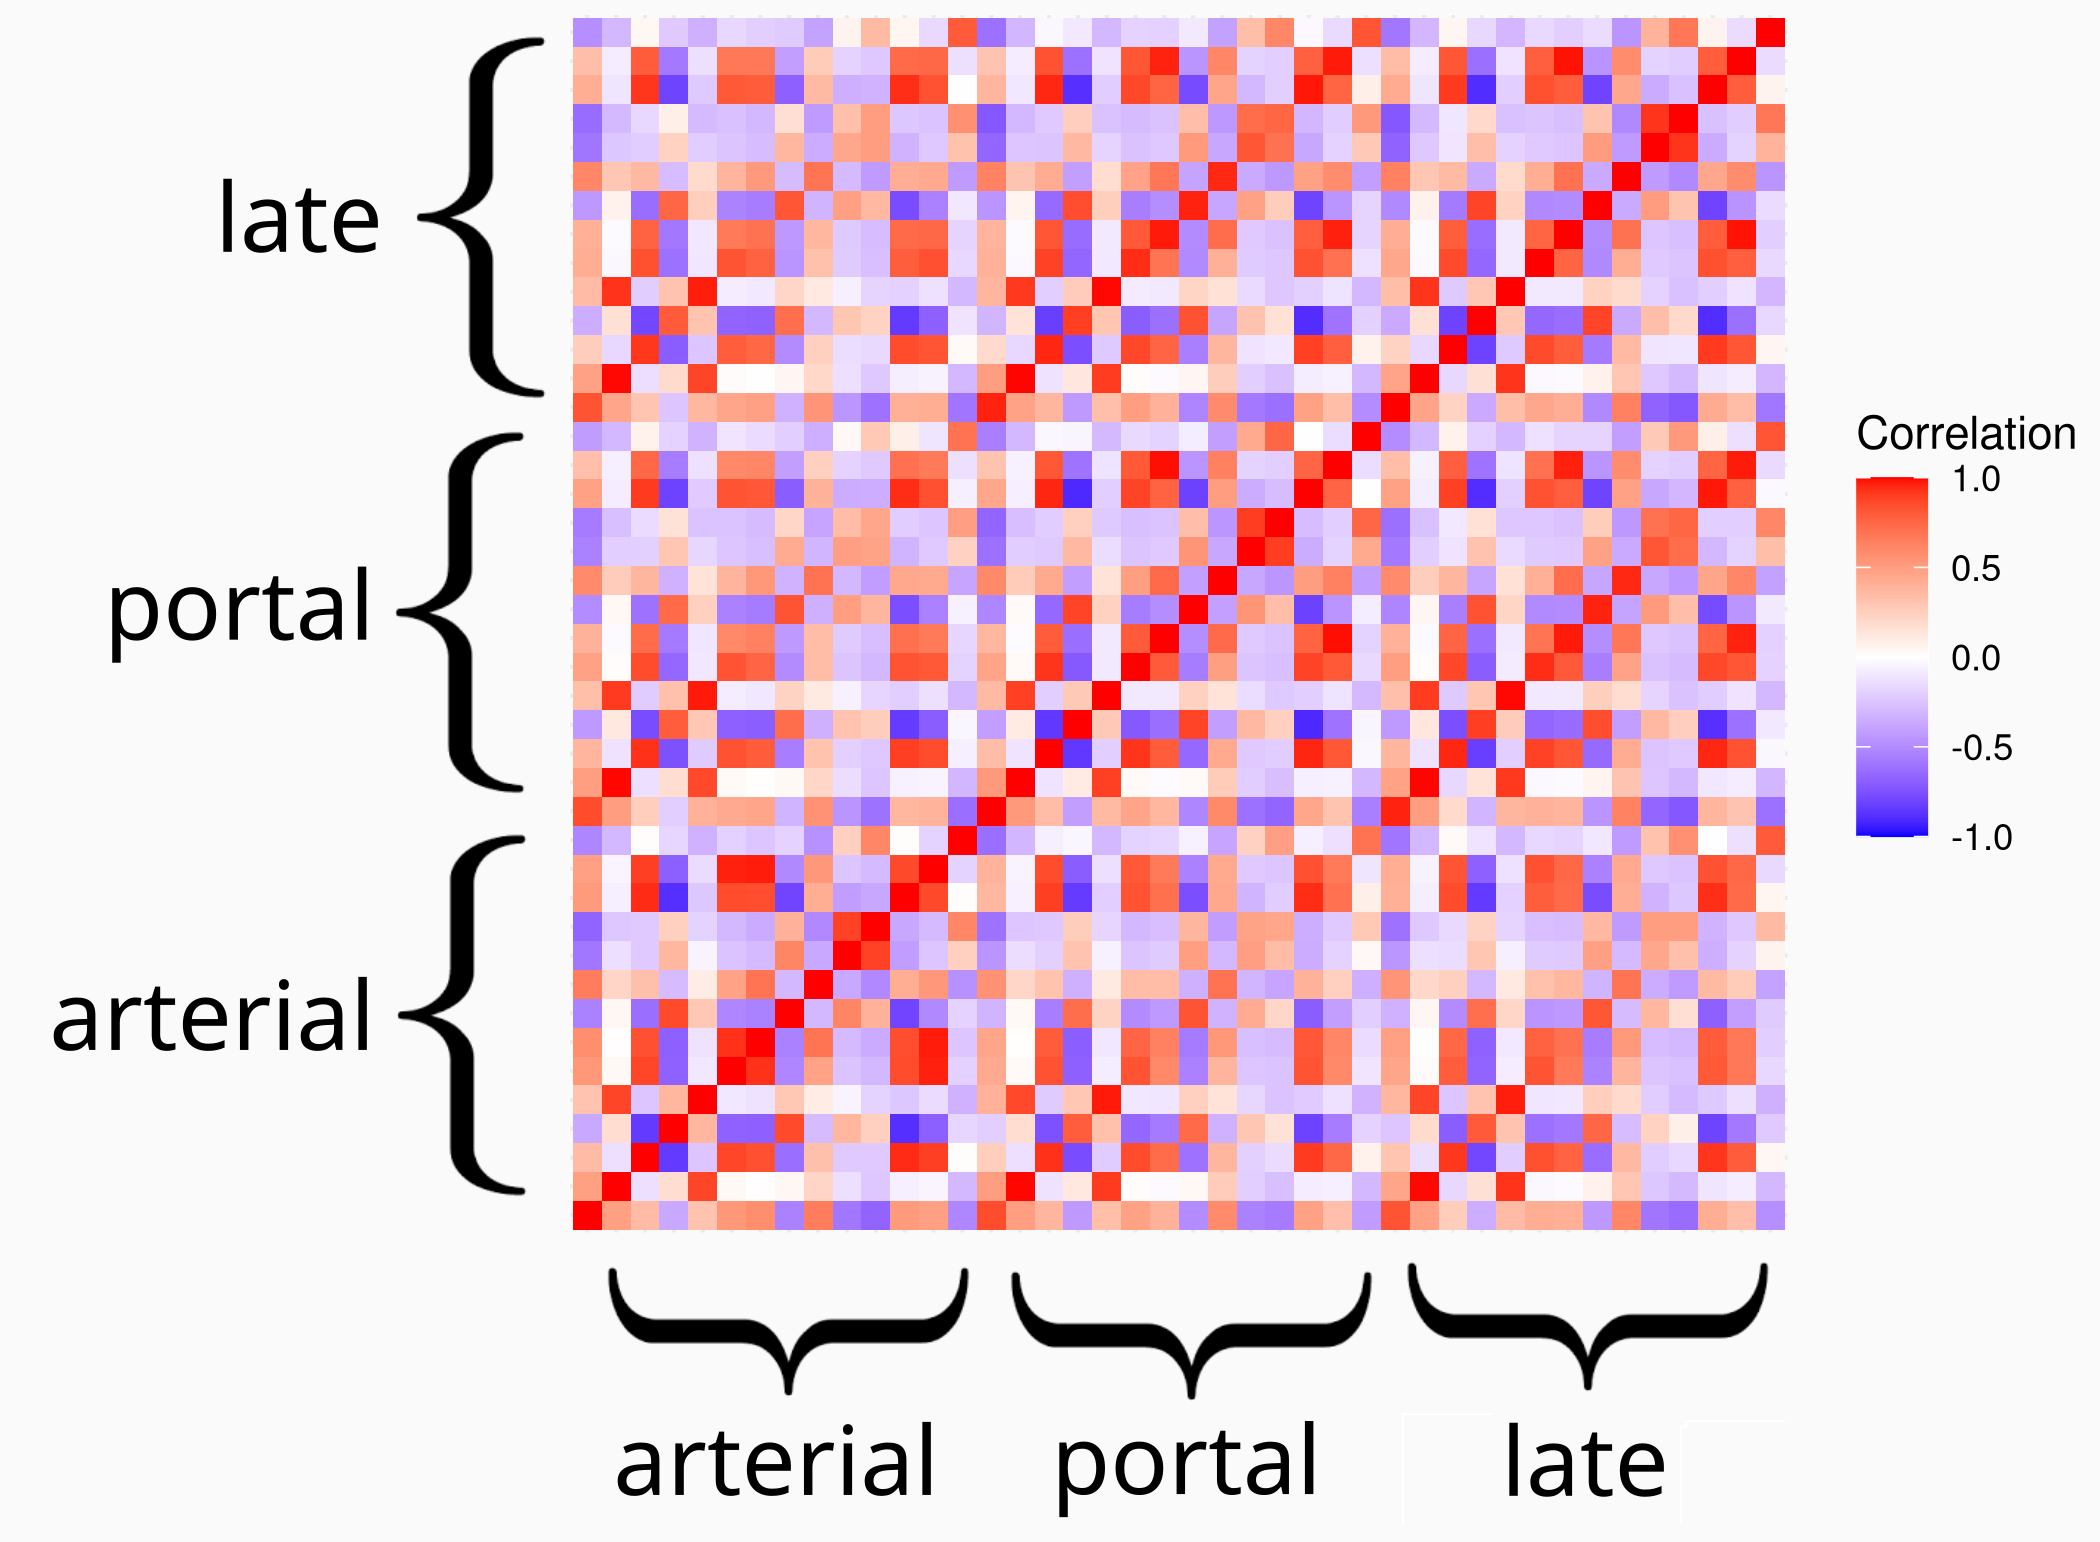
\includegraphics[scale = 0.1]{images/correlation.png}
%         \caption{Correlation matrix of the features relative to the Gray Level Dependence Matrix (GLDM)}
%     \end{figure}

% \end{frame}

\begin{frame}
    \frametitle{Liver tumors classification}
    \begin{center}
        \textbf{$\mathbf{6}^{\text{th}}$ most widespread cancer and $\mathbf{4}^{\text{th}}$ mortality cause by cancer}\\
    \end{center}
    Classification:
    \begin{itemize}
        \item Hepatocellular Carcinoma (HCC): $75\%$ of cases, resection often possible\\[10 pt]
        \item Cholangiocarcinoma (CCK): $6\%$ of cases, resection difficult (possible in $30\%$ of cases)\\[10 pt]
        \item Others: benign ($18 \%$ of cases) or Hepatoblastoma ($1 \%$ of cases)
    \end{itemize}

    Non invasive method: MRI images with injection of contrast agent
\end{frame}

\begin{frame}
    \frametitle{Some MRI images}
    \begin{figure}
        \centering
        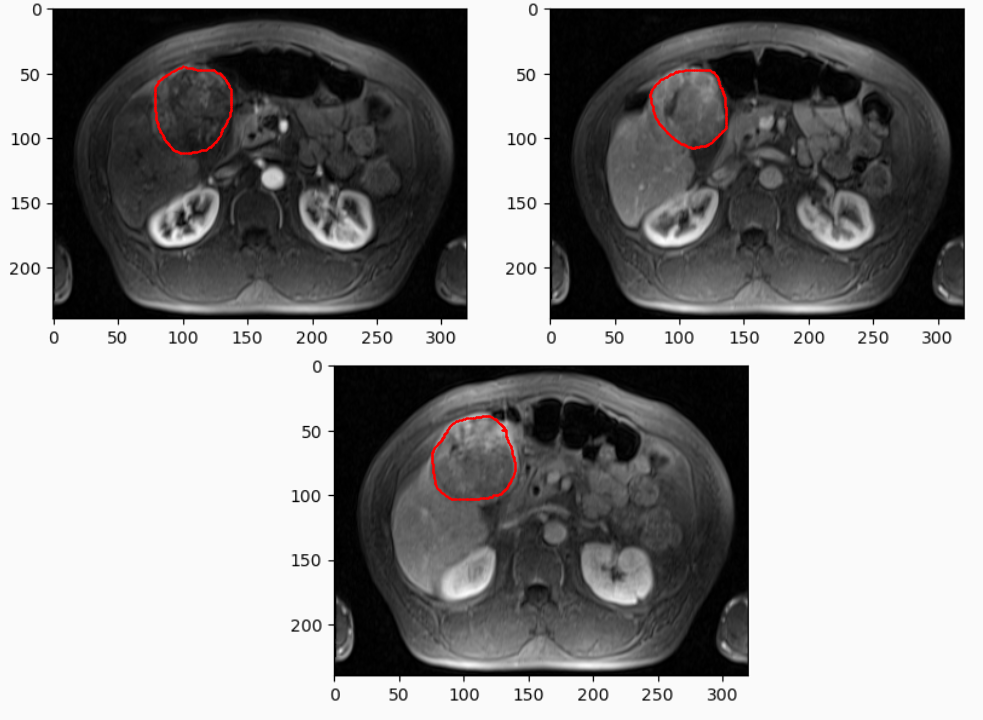
\includegraphics[scale = 0.215]{images/HCC.png}
        \caption{Example of MRI images of a HCC liver tumor (arterial, portal, late) from From Henri Mondor hospital: the 3 images look quite similar}
    \end{figure}
\end{frame}

\begin{frame}
    \frametitle{Some MRI images}
    \begin{figure}
        \centering
        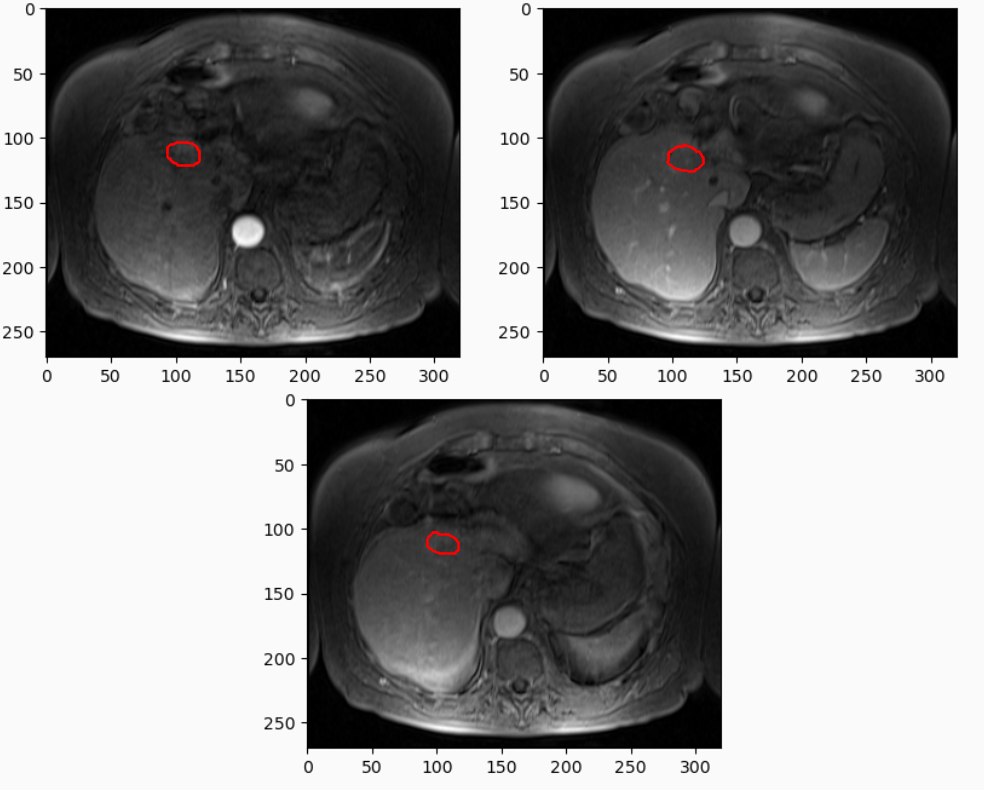
\includegraphics[scale = 0.215]{images/CCK.png}
        \caption{Example of MRI images of a CCK liver tumor (arterial, portal, late) from From Henri Mondor hospital}
    \end{figure}
\end{frame}


\begin{frame}
    \frametitle{Available data}

    $\bullet$ 3D MRI images of liver tumors taken at 3 times (arterial, portal, late) for each patient.\\[5 pt]
    \hspace{10 pt} - Same variables extracted from each of the 3 MRI images $\rightarrow$\\
    \hspace{10 pt} \textbf{tensor} \textbf{data}. \\
    \hspace{10 pt} - 3 blocks of MRI features: grey levels intensity, shape and\\
    \hspace{12 pt} texture $\rightarrow$ \textbf{multiblock data}\\[15 pt]

    $\bullet$ Clinical data:\\[5 pt]
    \hspace{10 pt} - Gender (63 men, 27 women) and age at disease (average $63$\\
    \hspace{12 pt} years old).\\
    \hspace{10 pt} - Form a separate block in the data



    
\end{frame}




\begin{frame}
    \frametitle{MRI features structured in a tensor data}
A given subject $i$ is represented by a horizontal slice $\mathbf{X}_i$ in the features tensor. 
    \begin{figure}
        \centering
        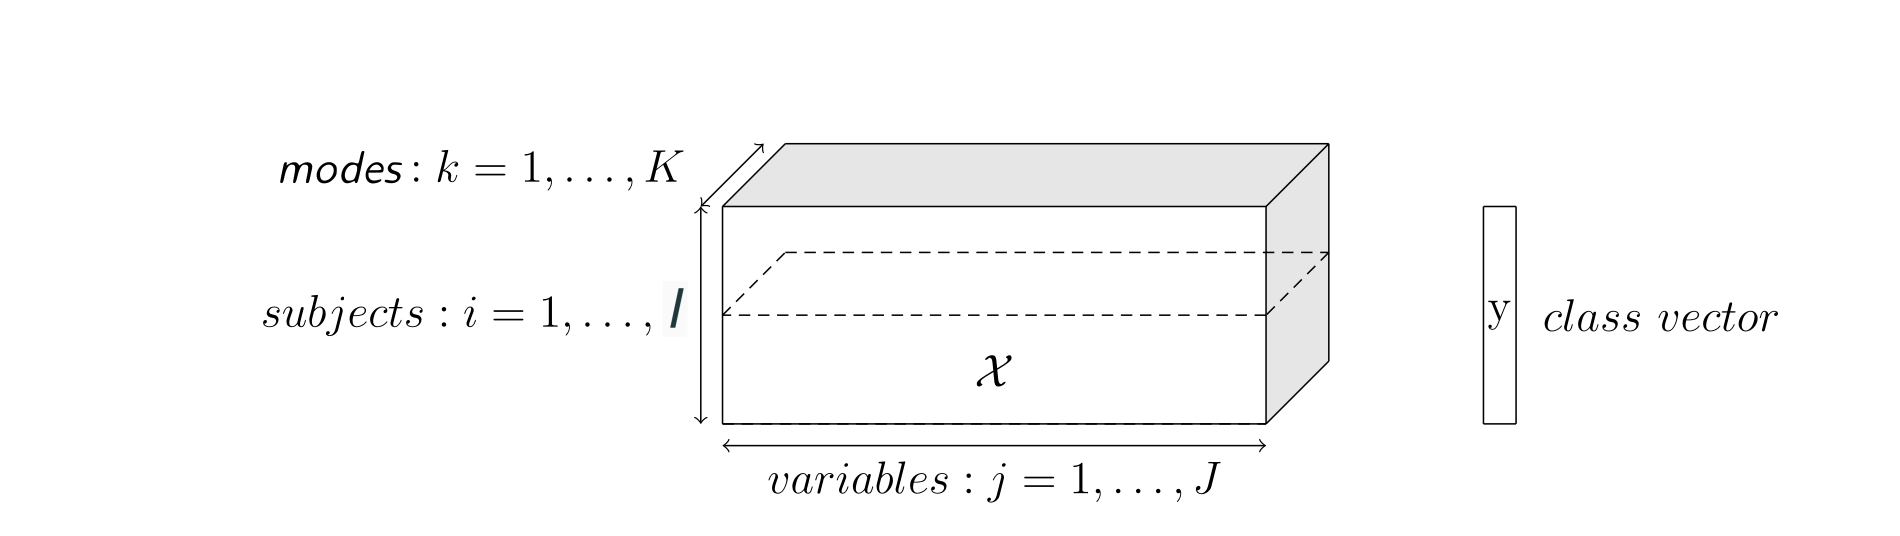
\includegraphics[scale = 0.23]{images/tensor_mode.png}
        \caption{Type of data: tensorial}
    \end{figure}

\end{frame}

\begin{frame}
    \frametitle{Multiblock data}
Each block is a tensor with its own structure.
    \begin{figure}
        \centering
        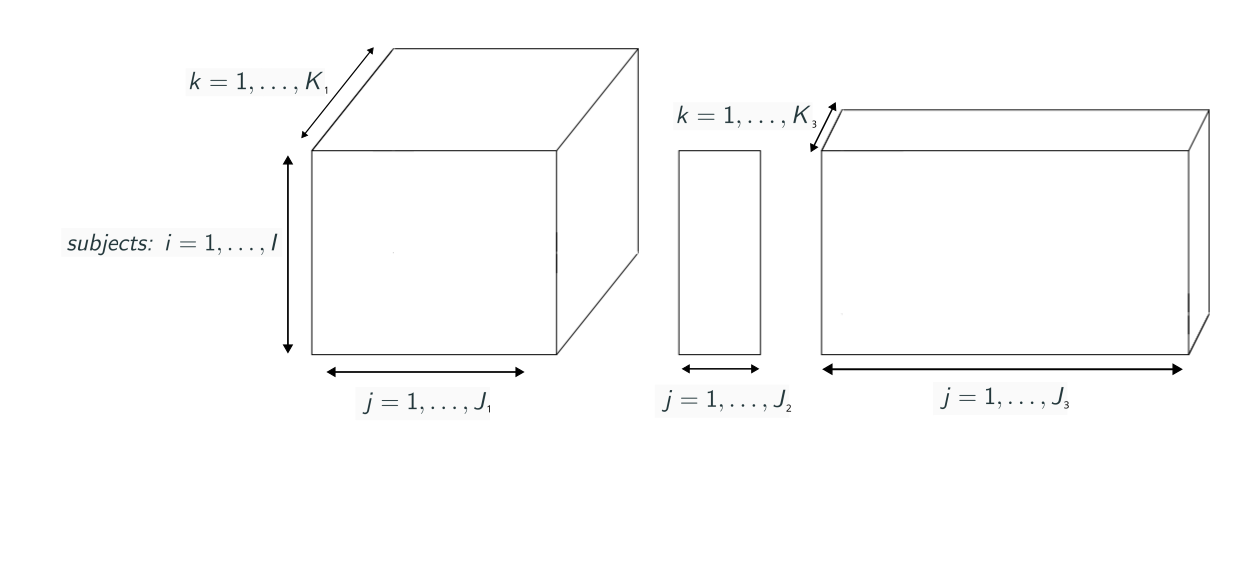
\includegraphics[scale = 0.25]{images/blocks.png}
        \caption{Type of data: multiblock}
    \end{figure}


\end{frame}

% \begin{frame}
%     \frametitle{Application example of real multiblock tensor data}
%     \textbf{classification of liver tumors through MRI}:\\[15 pt]
%     Same variables extracted from each MRI image at 3 times  (arterial, portal, late) $\rightarrow$ \textbf{tensor structure}\\[10 pt]

%     $\bullet$ MRI images in 3D of liver tumors. Information about grey levels, shape and correlations  $\rightarrow$ \textbf{multiblock structure}\\[5 pt]
%     $\bullet$ Also include univariate features: gender and age\\[10 pt]

%     \textbf{Conclusion}: \textbf{Multiblock tensor data} $\rightarrow$ train a tensor multiblock logistic regression model.
    
% \end{frame}


\begin{frame}
    \frametitle{Table of contents}
    \tableofcontents
\end{frame}

\section{Logistic model for tensor multiblock data}
\begin{frame}
\sectionpage
\end{frame}


\begin{frame}
    \frametitle{Logistic regression (recall)}
    Generalized linear model (GLM) for classification:\\[15 pt]
    \begin{tabular}{ll}
        $\mathbf{x}$ & \hspace{-8 pt}: feature vector (explanatory variable)\hspace{5 cm} \\[5 pt]
        $Y$ & \hspace{-8 pt}: binary response (explained variable) \hspace{10 cm}
    \end{tabular}
\vspace{5 pt}
\begin{block}{Likelihood for logistic regression}
$$P(Y = 1|\mathbf{x}) = \frac{\exp(\beta_0 + \mathbf{x}^T\hspace{-2 pt}\bm{\beta})}{1 + \exp(\beta_0 + \mathbf{x}^T\hspace{-2 pt}\bm{\beta})}$$
Defines a likelihood function $\mathcal{L}(\bm{\beta}) = \prod_{i = 1}^I P(Y_i = y_i|\mathbf{x_i})$ .
\end{block}

\end{frame}

\begin{frame}
    \frametitle{Naive approach for tensor data: unfolding}
    \begin{figure}
        \centering
        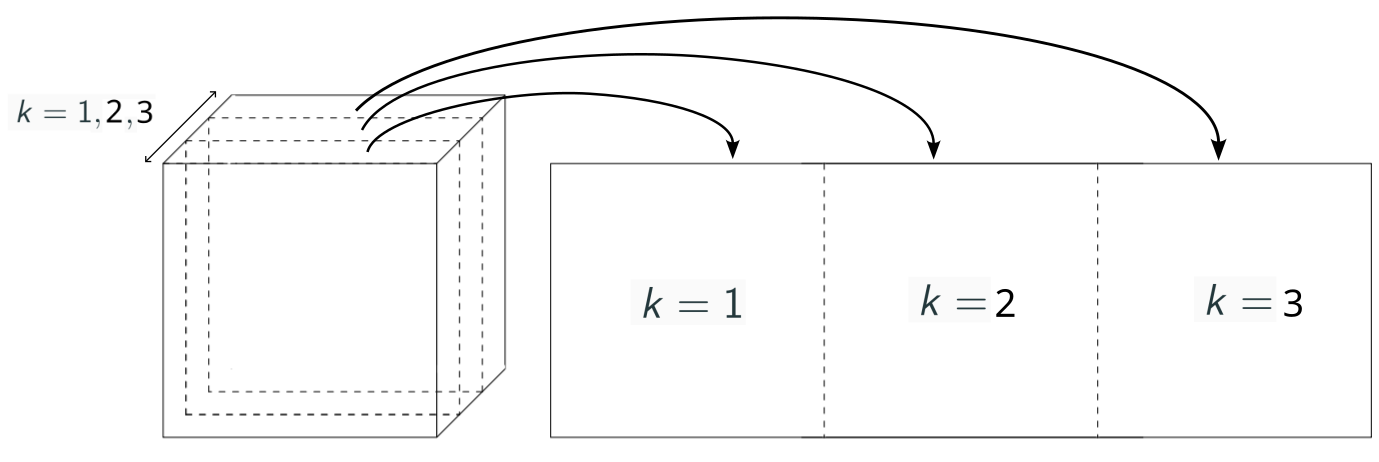
\includegraphics[scale = 0.15]{images/deplier.png}
        \caption{Unfolding a tensor}
    \end{figure}
    \begin{block}{Naive unfolding}
    $$\mathbf{B} = (\beta_{j,k})_{j \in \llbracket 1, J\rrbracket, k \in \llbracket 1, K\rrbracket} \rightarrow JK\text{ parameters to determine}$$ 
    $$\mathbf{x}^T \bm{\beta} \leadsto \sum\limits_{j,k} x_{j,k} \beta_{j,k} = \langle \, \mathbf{X} \, | \, \mathbf{B}\, \rangle$$
    \end{block}
    \textbf{Limitation}: No consideration of the tensor structure in the likelihood
    
    %Elimination of features without specific consideration for the same feature at other times/ other features at the same time.
    
\end{frame}

\begin{frame}
    \frametitle{Lasso penalization (recall)}
    To many features (vs $I$) $\rightarrow$ penalization to control variance of prediction (overfitting).\\[10 pt]
    Search for easily interpretable model $\rightarrow$ choice of lasso: 
    \begin{block}{Lasso}
    $$\text{penalization} = \lambda \lVert \bm{\beta} \rVert_1 \hspace{0.7 cm} (\lambda >0)$$
    Function to maximize : 
    $$ \text{penalized likelihood} =  \log(\mathcal{L}(\bm{\beta})) - \lambda \lVert \bm{\beta} \rVert_1 $$
    \end{block}
\vspace{5 pt}
    \textbf{Limitation}: No consideration of the tensor structure in the penalization.

    
\end{frame}


% \begin{frame}
%     \frametitle{Group lasso penalization}

%  \textbf{Common solution}: grouping regression coefficients together in the penalization.
%  $$ \sum\limits_{j,k} |\beta_{j,k}|\leadsto \sum\limits_{g = 1}^G \lVert \bm{\beta}^g \rVert_2 $$

%  Tendency to set regression coefficients to zero by entire blocks.\\[15 pt]

% \textbf{Limitation}: grouping either by mode or by variable, not both.

% \end{frame}

\begin{frame}
    \frametitle{Tensor regression model}
    \textbf{Idea}: each variable and mode has its own influence on the prediction \cite{multi_rank_1}.\\[10 pt]
    \begin{overprint}
    \onslide<1>
    \begin{figure}
        \centering
        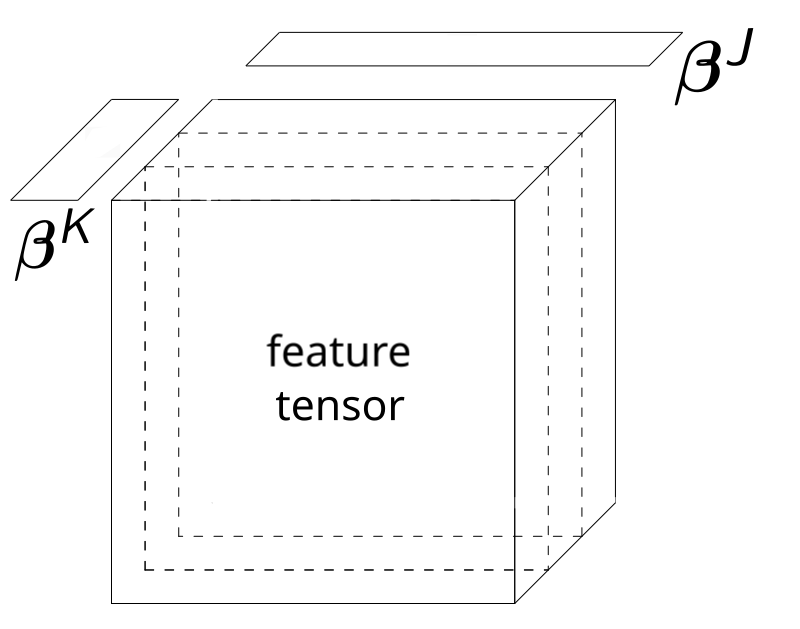
\includegraphics[scale = 0.3]{images/beta_tens.png}
        \caption{Tensor structure of $\mathbf{B}$}
    \end{figure}
    \onslide<2>
    \begin{block}{Proposed rank 1 model: outer product of vectors}
    For $J$ variables observed on $K$ modalities (e.g. times)
    $$ \mathbf{B} = \bm{\beta}^K \circ \bm{\beta}^J \hspace{0.7 cm}  (\beta_{j,k} = \beta_j^J\beta_{k}^{K})$$
    \end{block}
    $\beta_j^J$ : impact of variable $j$ \\[5 pt]
    $\beta_k^K$ : impact of modality $k$\\[10 pt]
    Only $J+K$ parameters to determine (instead of $JK$).
    
\end{overprint}
\end{frame}

\begin{frame}
    \frametitle{Limits of rank $1$}
    \vspace{10 pt}
    $\mathbf{B} = \bm{\beta}^K \circ \bm{\beta}^J$ \hspace{0.5 pt} implies a complete separation between columns and rows:
    \begin{figure}
            \centering
            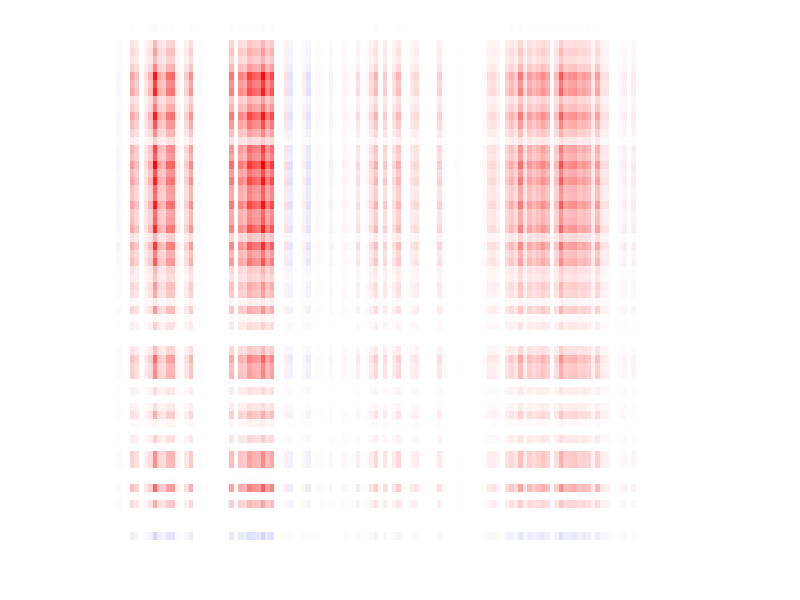
\includegraphics[width=0.5\textwidth]{images/picto_500/heatmap_logistic_multibloc_simu_500_multiway.png}
            \caption{\centering Heatmap of a rank 1 matrix: each pixel represents a number of the matrix $\mathbf{B}$ (from 0 in white to 1 in red)}
    \end{figure}
    \begin{center}
        This can be too simplistic.
    \end{center}


\end{frame}

\begin{frame}
    \frametitle{Extension to rank $R$ \cite{multi_rank_r}}
    \begin{block}{Rank R lasso penalized tensor model}
    \hspace{50 pt}Summing rank 1 together : $\mathbf{B} = \sum\limits_{r = 1}^R \bm{\beta}_{r}^J \circ \bm{\beta}_{r}^K$\\[-10 pt]
    $$ \text{lasso like penalization} \leadsto \lambda \sum\limits_{r = 1}^R  \lVert \bm{\beta}_r^J \circ \bm{\beta}_r^K \rVert_1  =  \lambda \sum\limits_{r = 1}^R\lVert \bm{\beta}_r^J \rVert_1 \lVert \bm{\beta}_r^K \rVert_1 $$
    \end{block}
    % $$\beta_{j,k}x_{j,k} = \left( \sum\limits_{r = 1}^R \beta_{j,r}^J\beta_{k,r}^K \right) x_{j,k} = \sum\limits_{r = 1}^R \beta_{j,r}^J\beta_{k,r}^K \hspace{1 pt} x_{j,k}$$
    \vspace{-10 pt}
\begin{figure}
        \centering
        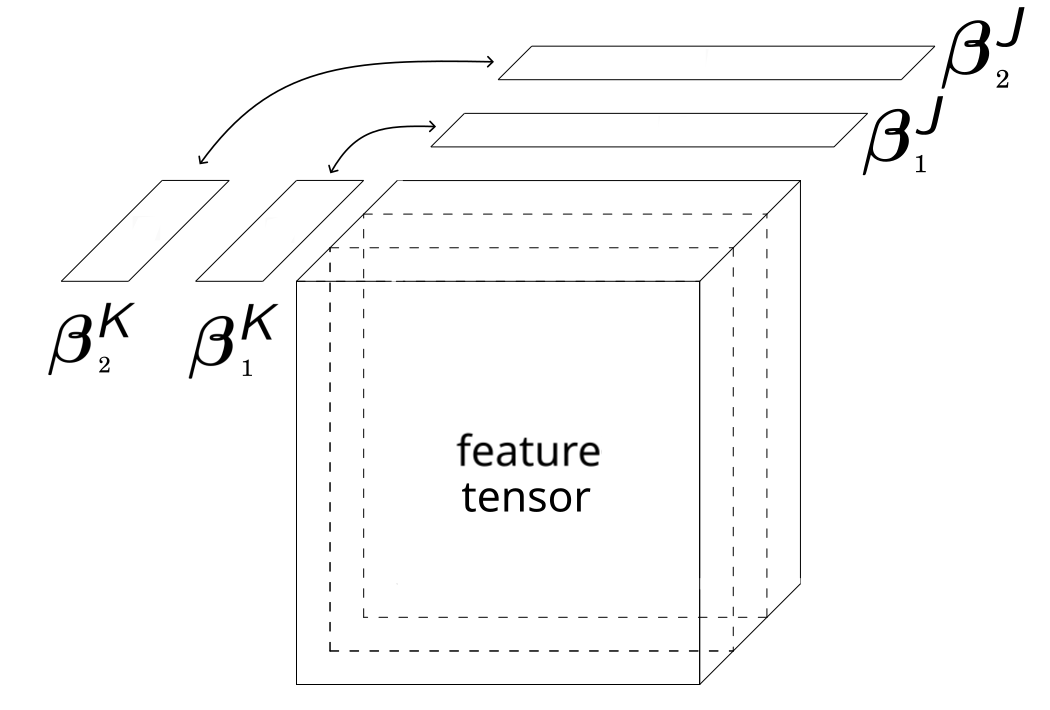
\includegraphics[scale=0.19]{images/beta_tens_R.png}
        \caption{Tensor structure of $\bm{\beta}$ for rank $2$}

\end{figure}

\end{frame}

\begin{frame}
 \frametitle{Blocks of variables (reminder)}
 \textbf{Aim}: GLM framework for multiblock tensor data.\\[10 pt]

 \begin{figure}
    \centering
    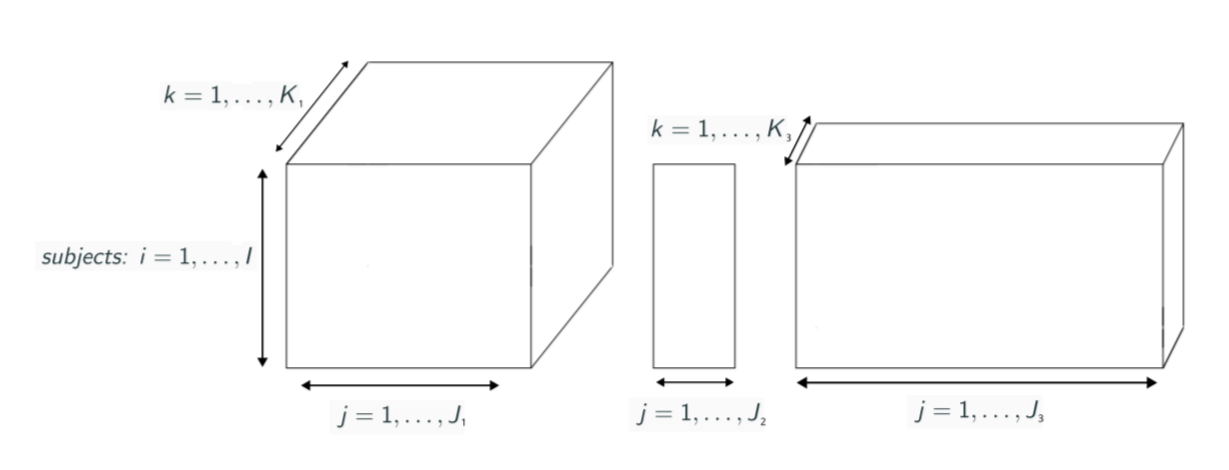
\includegraphics[scale = 0.33]{images/blocks_faux.png}
    \caption{One tensor per type of variable in multiblock data}
\end{figure}

\end{frame}

% \begin{frame}
%     \frametitle{Tensor model with blocks of variables}
%     If $K_1 = K_2$, blocks can be glued, but the structure is lost
%     \begin{figure}
%         \centering
%         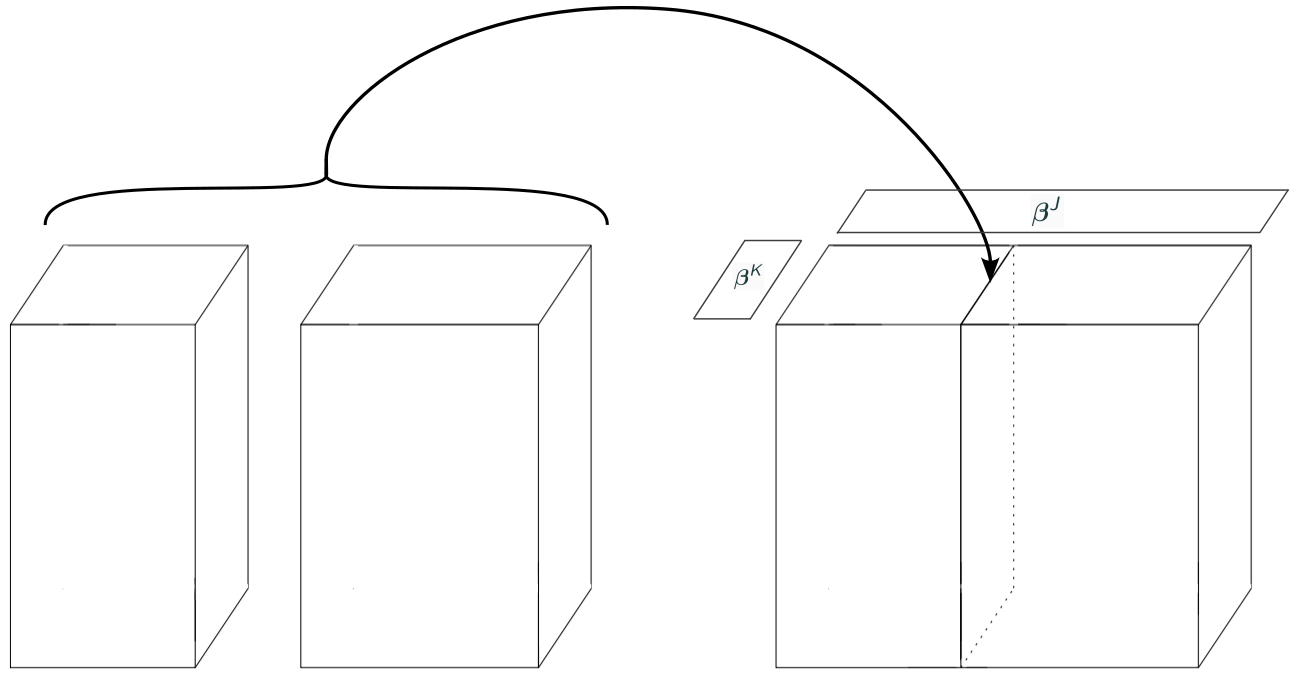
\includegraphics[scale = 0.2]{images/glue_blocks.png}
%         \caption{Tensor model with blocks of variables}
%     \end{figure}
% \end{frame}

\begin{frame}
    \frametitle{Logistic model for tensor multiblock data}
    \vspace{10 pt}
    \textbf{Solution}: giving each block its own $\bm{\beta}^J$ and $\bm{\beta}^K$\\[15 pt]
    \begin{figure}
        \centering
        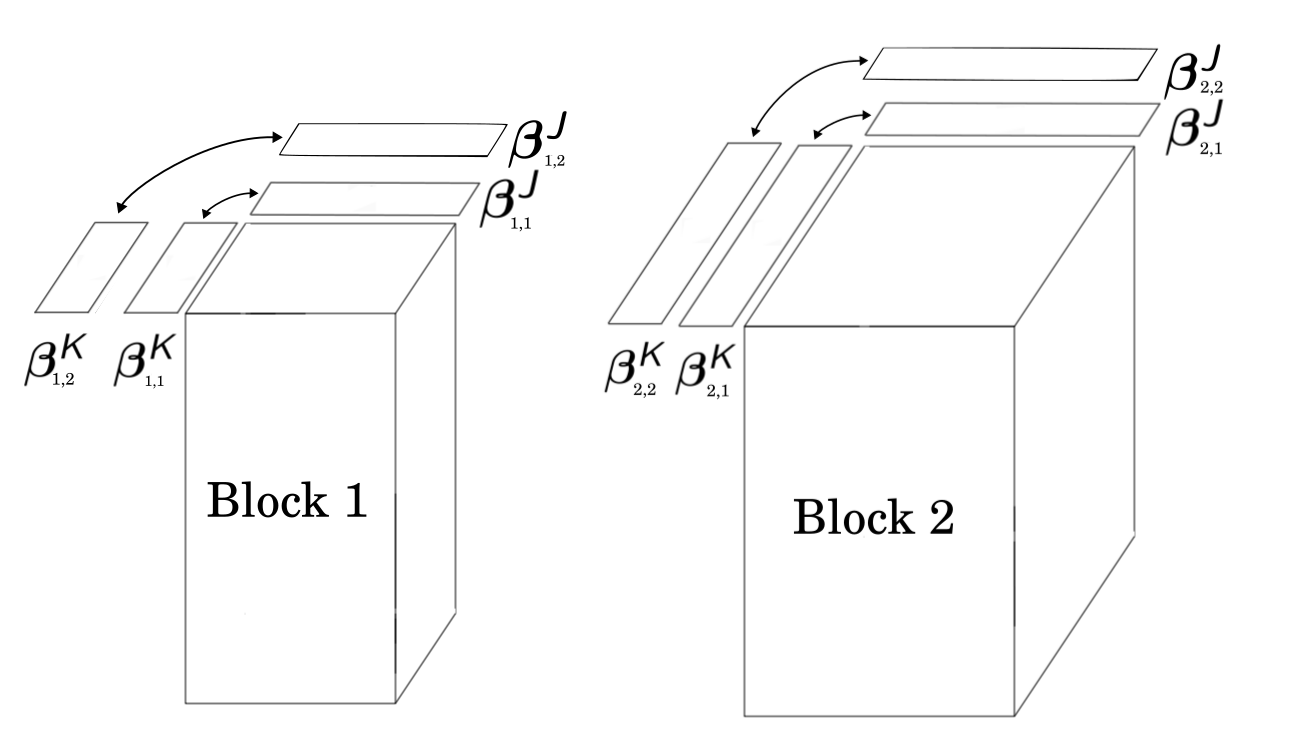
\includegraphics[scale = 0.26]{images/beta_blocks.png}
        \caption{Tensor multiblock model for rank 2}
    \end{figure}
\end{frame}

\begin{frame}
    \frametitle{Tensor multiblock logistic regression}
    \begin{block}{Scalar product for $L$ blocks}
        $$\mathbf{x}^T\bm{\beta} \leadsto \sum\limits_{\ell}\langle \,\mathbf{X}^\ell \, |\, \mathbf{B}_\ell \,\rangle  = \sum\limits_{\ell = 1}^L \sum\limits_{j,k} x_{j,k}^\ell(\beta_\ell)_{j,k}$$
       \end{block}

    \begin{block}{Regression coefficient for block $\ell$}
    
    $\mathbf{B}_\ell$ can have any rank $R_\ell$
    $$\mathbf{B}_\ell = \sum\limits_{r = 1}^{R_\ell} \bm{\beta}_{\ell,r}^J \circ \bm{\beta}_{\ell,r}^K $$
    \end{block}
    \begin{block}{Penalization}
        $$\text{Lasso like penalty} = \lambda \sum\limits_{\ell,r}\lVert \bm{\beta}_{\ell,r}^K \circ \bm{\beta}_{\ell,r}^J \rVert_1 = \lambda \sum\limits_{\ell,r}  \lVert \bm{\beta}_{\ell,r}^K \rVert_1 \lVert \bm{\beta}_{\ell,r}^J \rVert_1 $$
    \end{block}
\end{frame}

\section{Maximizing penalized likelihood}
\begin{frame}
\sectionpage
\end{frame}

\begin{frame}
\frametitle{likelihood term}
\begin{block}{Scalar product of $x$ and $\bm{\beta}$}
\begin{align*}
\mathbf{x}^T\bm{\beta} &\leadsto \sum\limits_{\ell,r,j,k} x_{j,k}^\ell(\beta_{\ell,r}^J)_j(\beta_{\ell,r}^K)_k\\[-5 pt]
&= \sum\limits_{\ell,r,j} \left(\sum\limits_{k}  x_{j,k}^\ell(\beta_{\ell,r}^{K})_k \, \right)(\beta_{\ell,r}^{J})_j
\end{align*}
\end{block}

\begin{block}{Partial optimization problem}
 Optimizing the likelihood along mode $J$ $\Leftrightarrow$ solving a logistic regression on weighted aggregated data $\sum\limits_{k}  x_{j,k}^\ell(\beta_{\ell,r}^{K})_k $
\end{block}
\begin{block}{Algorihm}
Similar result for mode $K$. Possibility to optimize the likelihood by alternating between modes (can be easily adapted for lasso penalization)
\end{block}
% If a mode is inexistent in a block, renumber the modes of that block to perform the optimization on another (existing) mode of this block.

\end{frame}




\section{Tests on simulated data and application to liver tumor classification}  
\begin{frame}
  \sectionpage
\end{frame}


\begin{frame}
    \frametitle{Data generation: example in 2D}

    \begin{figure}
        \centering
        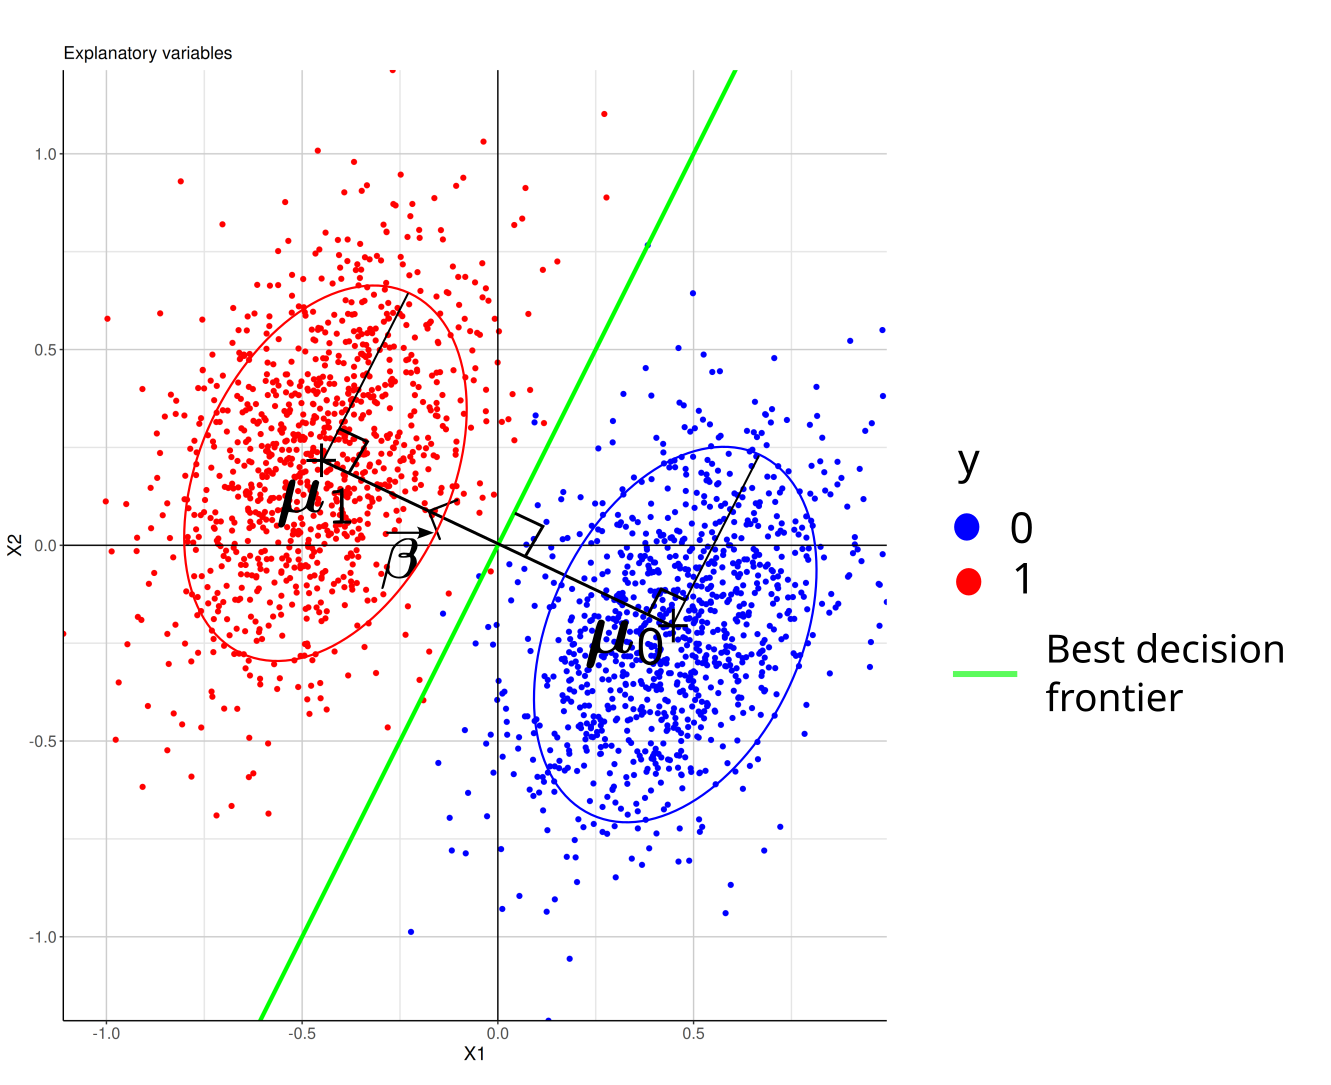
\includegraphics[scale = 0.2]{images/2D_better.png}
        \caption{Example of explanatory variables for $\bm{\beta} = (-2,1)$}
    \end{figure}
    Possibility to choose $(\sigma_\beta,\sigma_{\text{noise}})$ to define the problem difficulty.
\end{frame}

\begin{frame}
    \frametitle{AUC on simulated data}
    \begin{figure}
        \begin{table}[H]
            \centering
            \caption{Cross validated AUC for each model on simulated data for 3000 individuals}
            \label{tab:result_simul}
            \renewcommand{\arraystretch}{1.2} 
            \begin{adjustbox}{center}
            \begin{tabular}{|>{\centering\arraybackslash}m{1.7cm}|>{\centering\arraybackslash}m{1.1cm}|>{\centering\arraybackslash}m{1.1cm}|>{\centering\arraybackslash}m{1.1cm}|>{\centering\arraybackslash}m{1.1cm}|>{\centering\arraybackslash}m{1.1cm}|>{\centering\arraybackslash}m{1.1cm}|}
                \cline{1-7}
                $(\sigma_{\bm{\beta}}, \sigma_{\text{noise}})$ & lasso & g.l. (blocks) & g.l. (mode)& g.l. (var) & tensor & tensor blocks\\
                \cline{1-7} 
                (0.1,0.5) & 0.83 & 0.86 & 0.94 & 0.94 & 0.99 & 0.99 \\
                \cline{1-7}
                (0.1,0.8) & 0.63 & 0.64 & 0.68 & 0.68 & 0.93 & 0.99 \\
                \cline{1-7}
            \end{tabular}
        \end{adjustbox}
        \end{table}
    \end{figure}
    
    \begin{figure}
        \centering
        \begin{minipage}{0.45\textwidth}
            \centering
            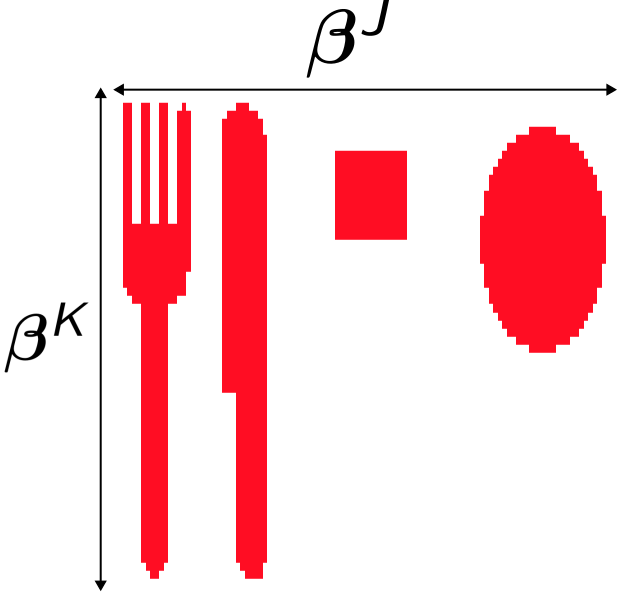
\includegraphics[scale = 0.17]{images/3_picto.png}
            \caption{Pictogram for non multiblock models}
        \end{minipage}
        \begin{minipage}{0.45\textwidth}
            \centering
        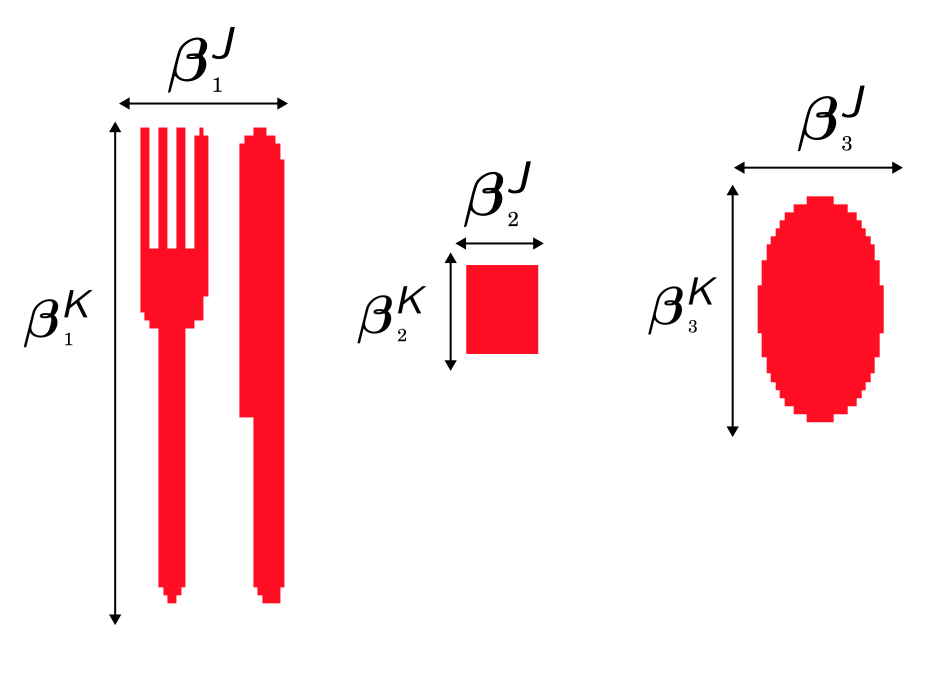
\includegraphics[scale = 0.17]{images/3_picto_sepa.png}
        \caption{Pictogram for tensor multiblock model}
    \end{minipage}
    \end{figure}

\end{frame}

\begin{frame}

    \frametitle{Reconstructed $\bm{\beta}$}
    \begin{figure}[H]
        \centering
        \begin{minipage}{0.30\textwidth}
            \centering
            \subfloat[lasso $(\sigma_{\bm{\beta}}, \sigma_{\text{noise}}) = (0.1,0.5) $\label{fig:3000simple}]{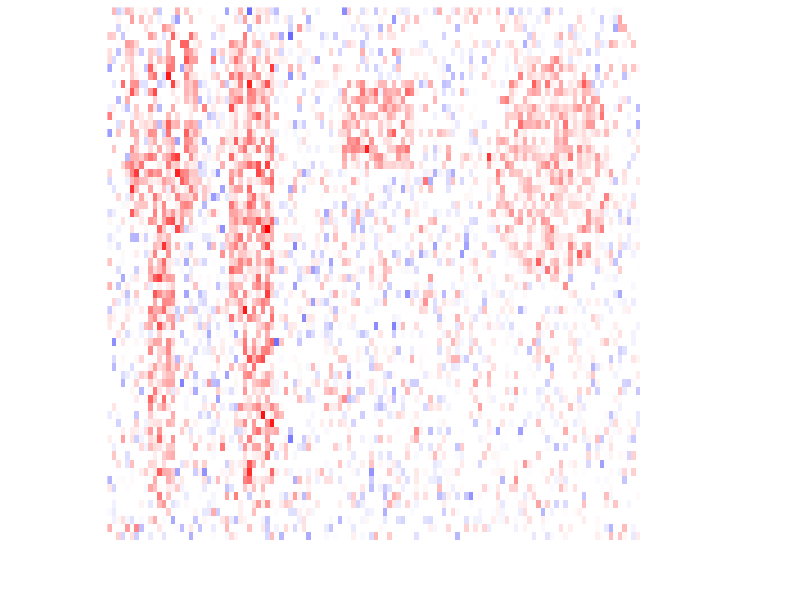
\includegraphics[width=\textwidth]{images/heatmap_logistique_simple_simu_4000.png}}
        \end{minipage}
        \begin{minipage}{0.30\textwidth}
            \centering
            \subfloat[tensor $R: 10$ $(\sigma_{\bm{\beta}}, \sigma_{\text{noise}}) = (0.1,0.5) $\label{fig:3000simple}]{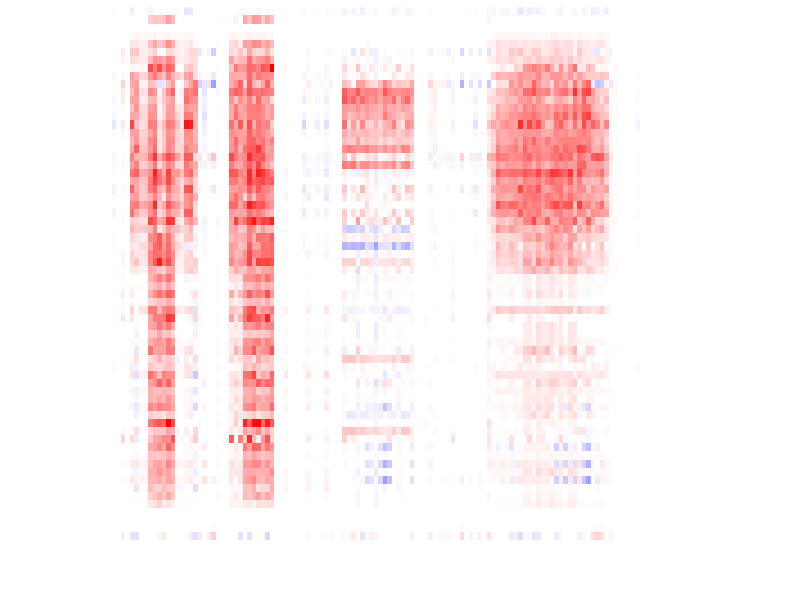
\includegraphics[width=\textwidth]{images/heatmap_logistic_multibloc_simu_4000_multiway.png}}
        \end{minipage}
        \begin{minipage}{0.30\textwidth}
            \centering
            \subfloat[T.M. $R: (12,1,10)$ $(\sigma_{\bm{\beta}}, \sigma_{\text{noise}}) = (0.1,0.5) $\label{fig:multiblock}]{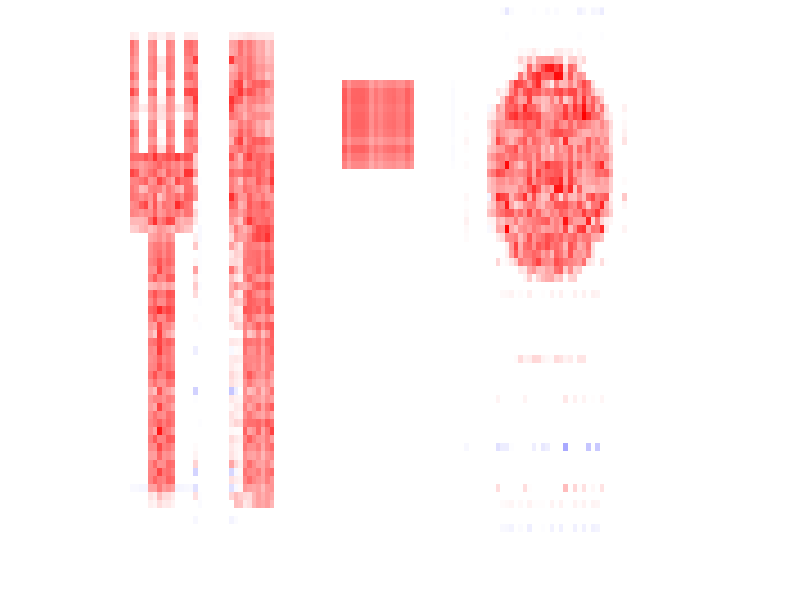
\includegraphics[width=\textwidth]{images/heatmap_logistic_multibloc_simu_4000.png}}
        \end{minipage}
        \begin{minipage}{0.30\textwidth}
            \centering
            \subfloat[lasso $(\sigma_{\bm{\beta}}, \sigma_{\text{noise}}) = (0.1,0.8) $\label{fig:easy_multiblock}]{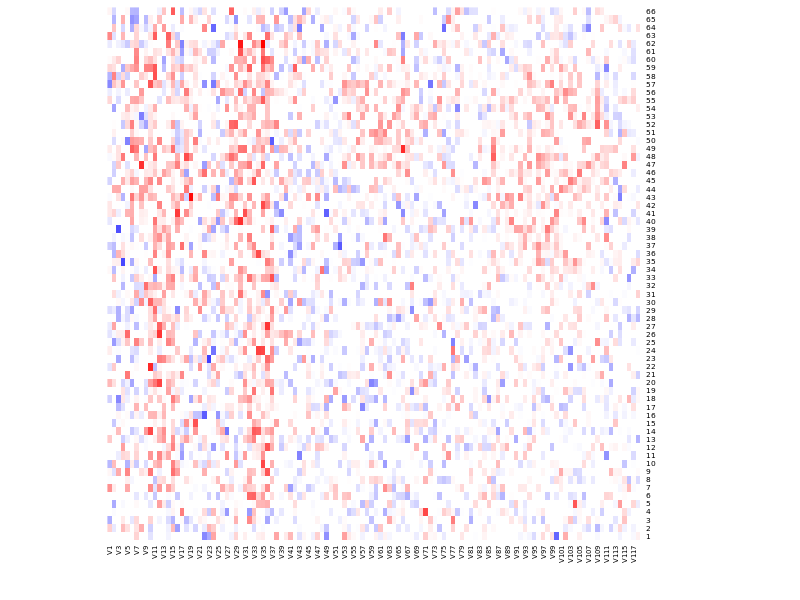
\includegraphics[width=\textwidth]{images/heatmap_logistique_simple_simu_medium_easy.png}}
        \end{minipage}
        \begin{minipage}{0.30\textwidth}
            \centering
            \subfloat[tensor $R: 10$ $(\sigma_{\bm{\beta}}, \sigma_{\text{noise}}) = (0.1,0.8) $\label{fig:easy_multiway}]{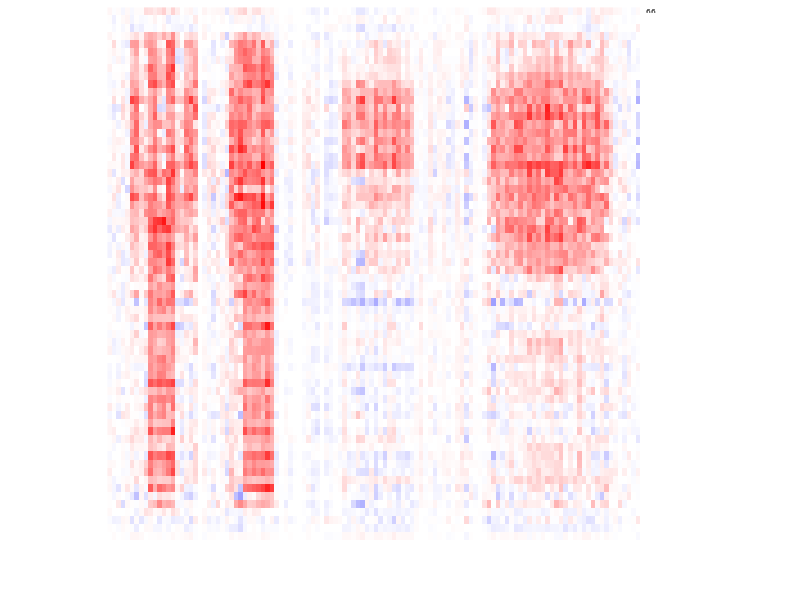
\includegraphics[width=\textwidth]{images/heatmap_logistic_multibloc_simu_4000_medium_easy_multiway.png}}
        \end{minipage}
        \begin{minipage}{0.30\textwidth}
            \centering
            \subfloat[T.M. $R: (6,1,1)$ $(\sigma_{\bm{\beta}}, \sigma_{\text{noise}}) = (0.1,0.8) $\label{fig:easy_multiblock}]{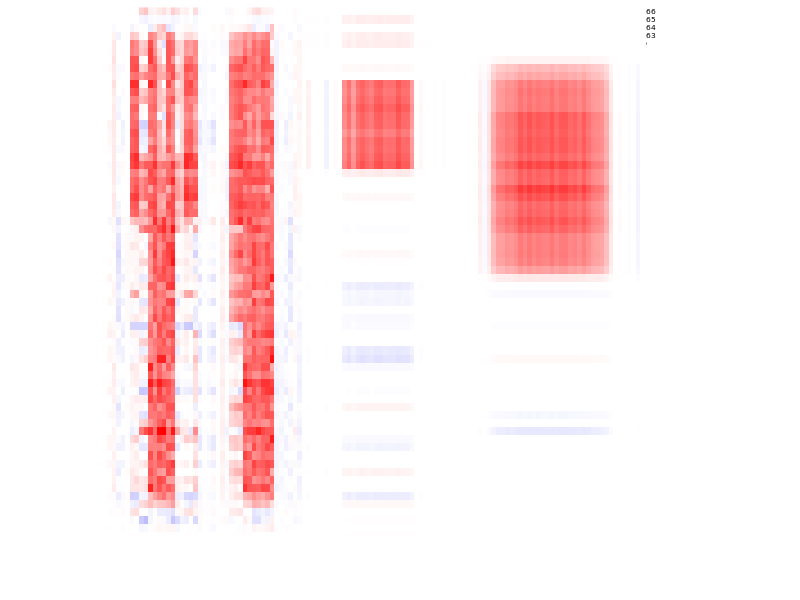
\includegraphics[width=\textwidth]{images/heatmap_logistic_multibloc_simu_4000_medium_easy.png}}
        \end{minipage}
    \end{figure}
\end{frame}

% \begin{frame}
%     \frametitle{Interpretation of the results}
%     Better reconstruction by tensor multiblock logistic model.\\[10 pt]
%     Performance (AUC) in adequation with quality of reconstruction (because small changes in $\bm{\beta}$ $\leadsto$ big changes in the classification, when $\sigma_{\text{noise}}$ increases).\\[10 pt]
%     Efficient sparse (low rank) approximation of pictograms by tensor multiblock logistic model in contrast with simple tensor model.\\[10 pt]
%     Tendency to choose rank $1$ for both tensor model when too few data (or too high noise).

% \end{frame}


% \begin{frame}
%     \frametitle{Feature extraction with pyradiomics \cite{pyradio}}
%     Extraction of $\simeq  100$ features (about intensities, shape, texture) for each $2$D or $3$D image.\\[10 pt]
%     \begin{figure}
%         \centering
%         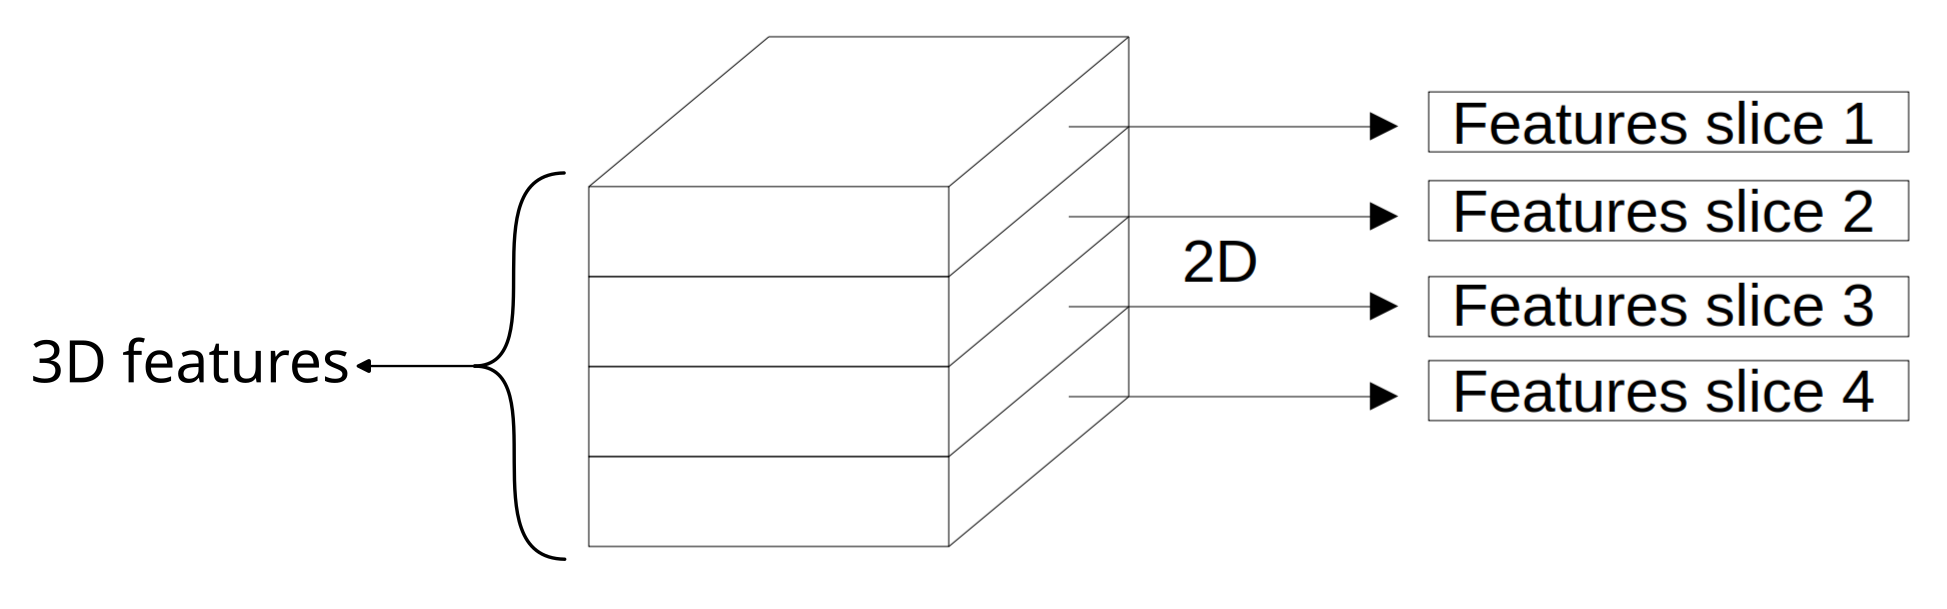
\includegraphics[scale = 0.15]{images/features.png}
%         \caption{Feature extraction with pyradiomics for an MRI image composed of $4$ slices}
%     \end{figure}
% \end{frame}

% \begin{frame}
%     \frametitle{Feature extraction in 3D}
%     Each radio $\rightarrow$ 1 particular spacing along $(x,y,z)$\\[10 pt]
%     \textbf{But} : Calculations of pyradiomics only use voxels (= 3D pixels).\\[10 pt]
%     Not always meaningful if the scale changes at each radio (e.g. for Gray Level Run Length Matrix, based on number alignments of voxels of same intensity)\\[10 pt]
%     \textbf{Solution}: Standardize the spacing along $(x,y,z)$. Allowed by resampling (interpolation) of the image.
% \end{frame}

% \begin{frame}
%     \frametitle{Feature extraction in 2D}
%     \vspace{5 pt}
%     Slices along z axis $\rightarrow$ same spacing along $(x,y)$\\[5 pt]
%     \textbf{Difficulty} Tumors are of variable locations, sizes and shapes in the frontal plane (front - back plane)
%     \begin{figure}
%         \begin{minipage}{0.45\textwidth}
%             \centering
%             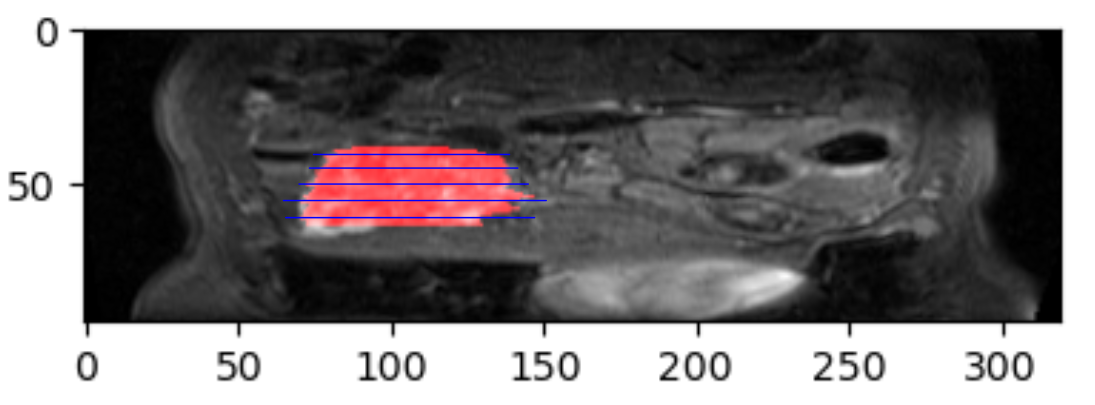
\includegraphics[scale = 0.125]{images/slices_big.png}
%             \caption{Extracting 5 slices in a big tumor}
%         \end{minipage}
%         \hspace{0.03\textwidth} 
%         \begin{minipage}{0.45\textwidth}
%             \centering
%             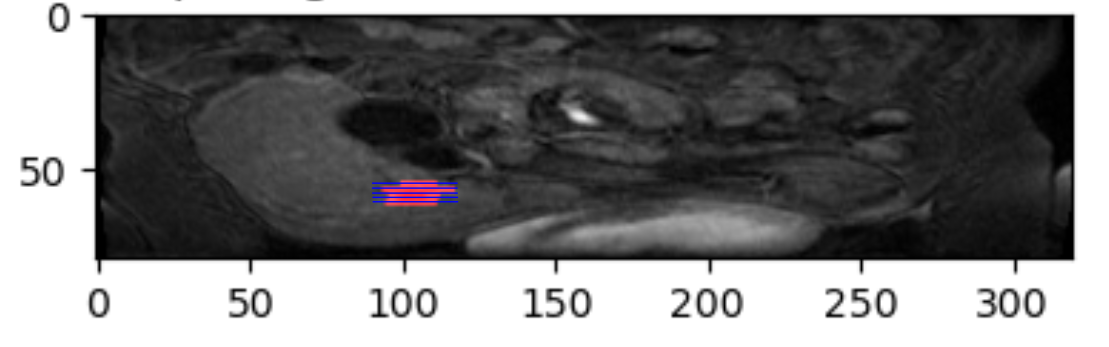
\includegraphics[scale = 0.18]{images/slices_small.png}
%             \caption{Extracting 5 slices in a small tumor}
%         \end{minipage}
%     \end{figure}
% \end{frame}

% \begin{frame}
%     \frametitle{Feature extraction in 2D}
%     Every slice not equally informative:
%     \begin{figure}
%         \centering
%         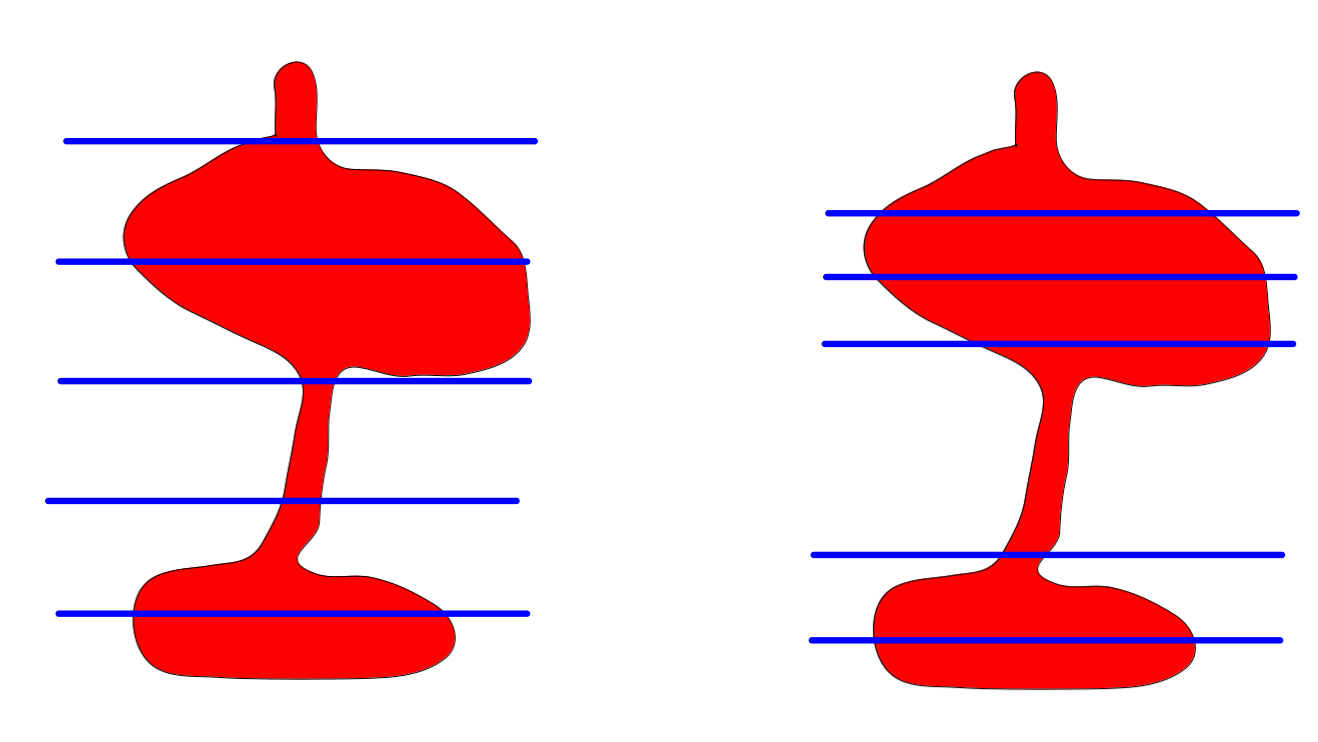
\includegraphics[scale = 0.2]{images/bad_shape.png}
%         \caption{Slicing relative to the depth vs. relative to the volume travelled in the tumor}
%     \end{figure}
% \end{frame}

% \begin{frame}
%     \frametitle{Feature extraction in 2D}
%     \textbf{Solution}: Selecting $5$ slices equally spaced along the cumulated volume axis
%     \begin{figure}
%         \centering
%         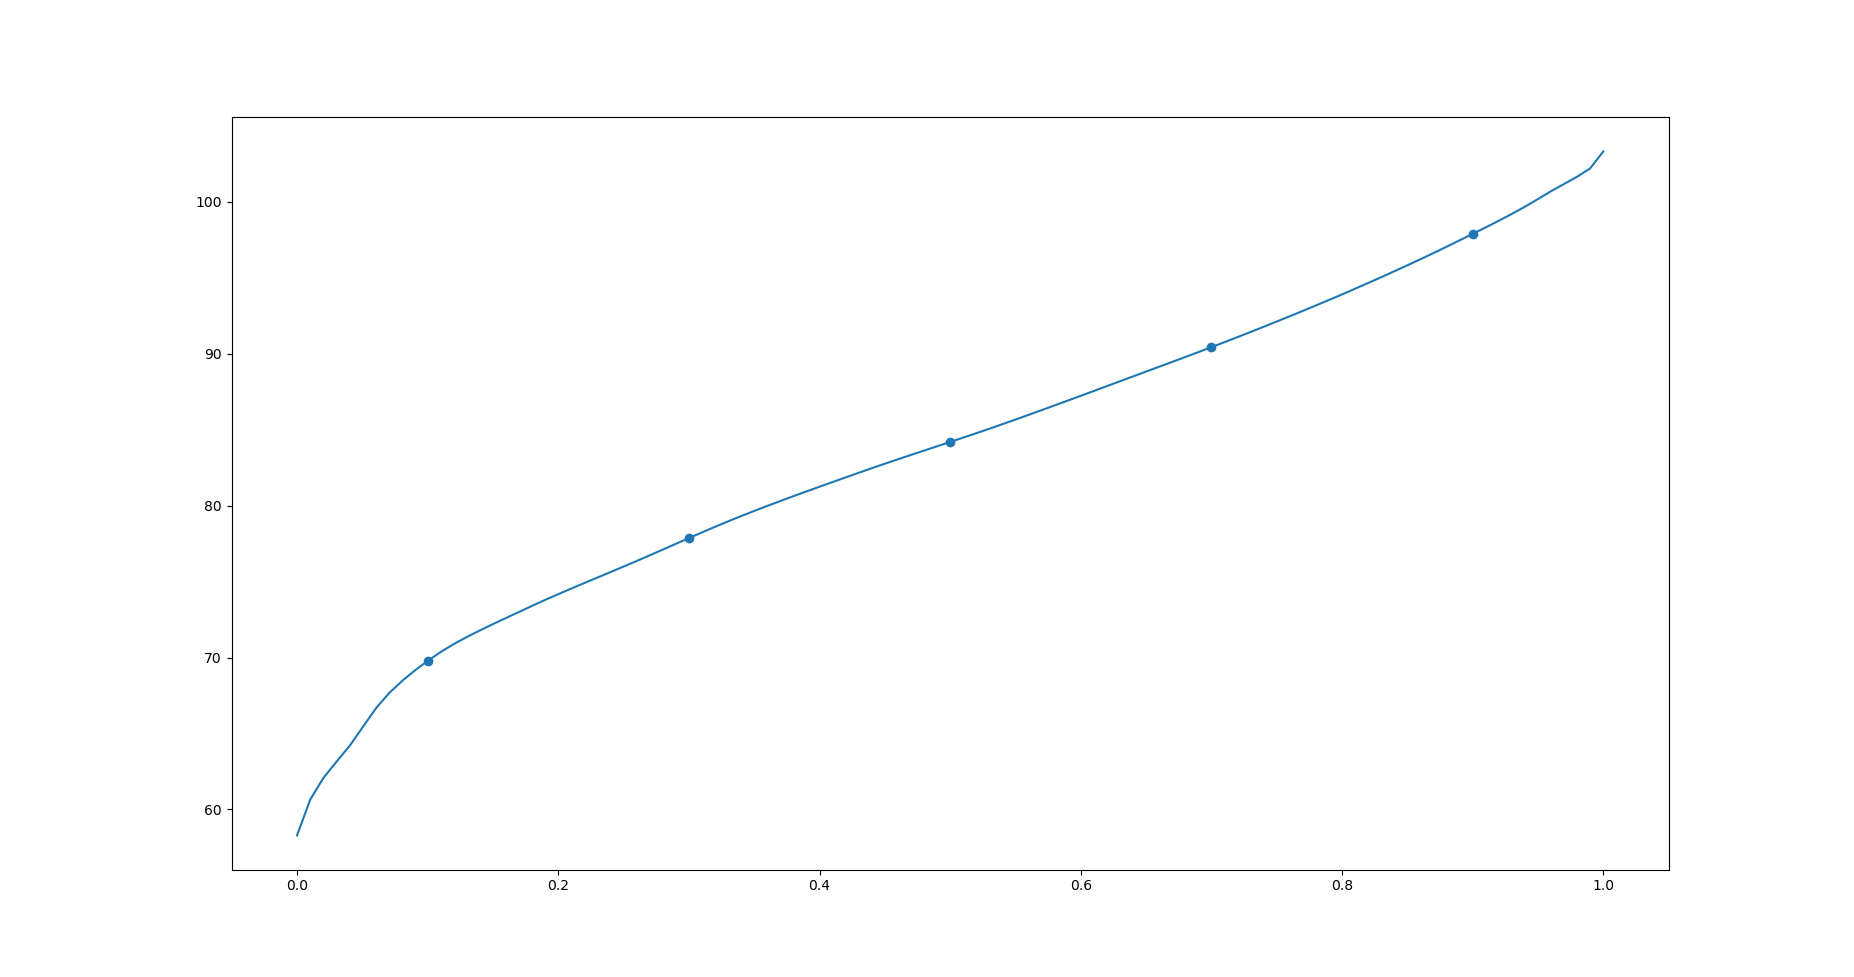
\includegraphics[scale = 0.15]{images/curve_points.png}
%         \caption{Curve of the depth travelled in the liver  (in $mm$) as a function of the standardized cumulated volume of the tumor. The points represent the selected slices.}
%     \end{figure}
% \end{frame}

\begin{frame}
    \frametitle{Results on liver tumor data}
    \begin{table}[H]
        \centering
        \label{tab:result_real}
        \renewcommand{\arraystretch}{1.2} 
        \begin{adjustbox}{center}
        \begin{tabular}{|>{\centering\arraybackslash}m{1.1cm}|>{\centering\arraybackslash}m{1.8cm}|>{\centering\arraybackslash}m{1.8cm}|>{\centering\arraybackslash}m{1.8cm}|>{\centering\arraybackslash}m{1.1cm}|>{\centering\arraybackslash}m{1.1cm}|}
            \cline{1-6}
             lasso & group lasso (block) & group lasso (time)& group lasso (var) & tensor & tensor blocks\\
            \cline{1-6} 
             $0.74 \pm 0.04$& $0.78 \pm 0.03$ & $0.76 \pm 0.03$ & $0.73 \pm 0.03$ & $0.77 \pm 0.03$ & $0.77 \pm 0.03$ \\
            \cline{1-6}
        \end{tabular}
        
    \end{adjustbox}
    \parbox{0.9\textwidth}{
    \vspace{0.2 cm}    
    \centering \small Cross validated AUC on 3D real data}
    \vspace{0.3 cm}
    \end{table}

    Performances of tensor models similar to those of the best model (here group lasso, with grouping of features by block), but better explainability (less parameters to determine).
\end{frame}

\begin{frame}
    \frametitle{Conclusion}
    $\bullet$ State of the art performances.\\[15 pt]
    $\bullet$ Better than state of the art in simulated data.\\[15 pt]
    $\bullet$ Scales better than regular logistic regression for high order tensors.\\[15 pt]
    $\bullet$ Lowers the complexity of the regression model \\[15 pt]
    $\bullet$ Good interpretability (sparse + displays importance of each block, mode and variable in $\bm{\beta}$).

\end{frame}

% \subsection{latest data}

% \begin{frame}
%     \frametitle{Latest data}
%     12 binary features determined by radiologists (late enhancement, non peripheral washout etc...) + sex and existence of chronical disease\\[10 pt]
%     With lasso model:
%     \begin{itemize}
%         \item AUC: $0.97 \pm 0.02$\\[10 pt]
%         \item balanced accuracy: $0.88 \pm 0.05$
%         \end{itemize}
%     Would be interesting to test other models...
% \end{frame}

% \begin{frame}
%     \frametitle{Feature importance}
%     \begin{figure}
%         \centering
%         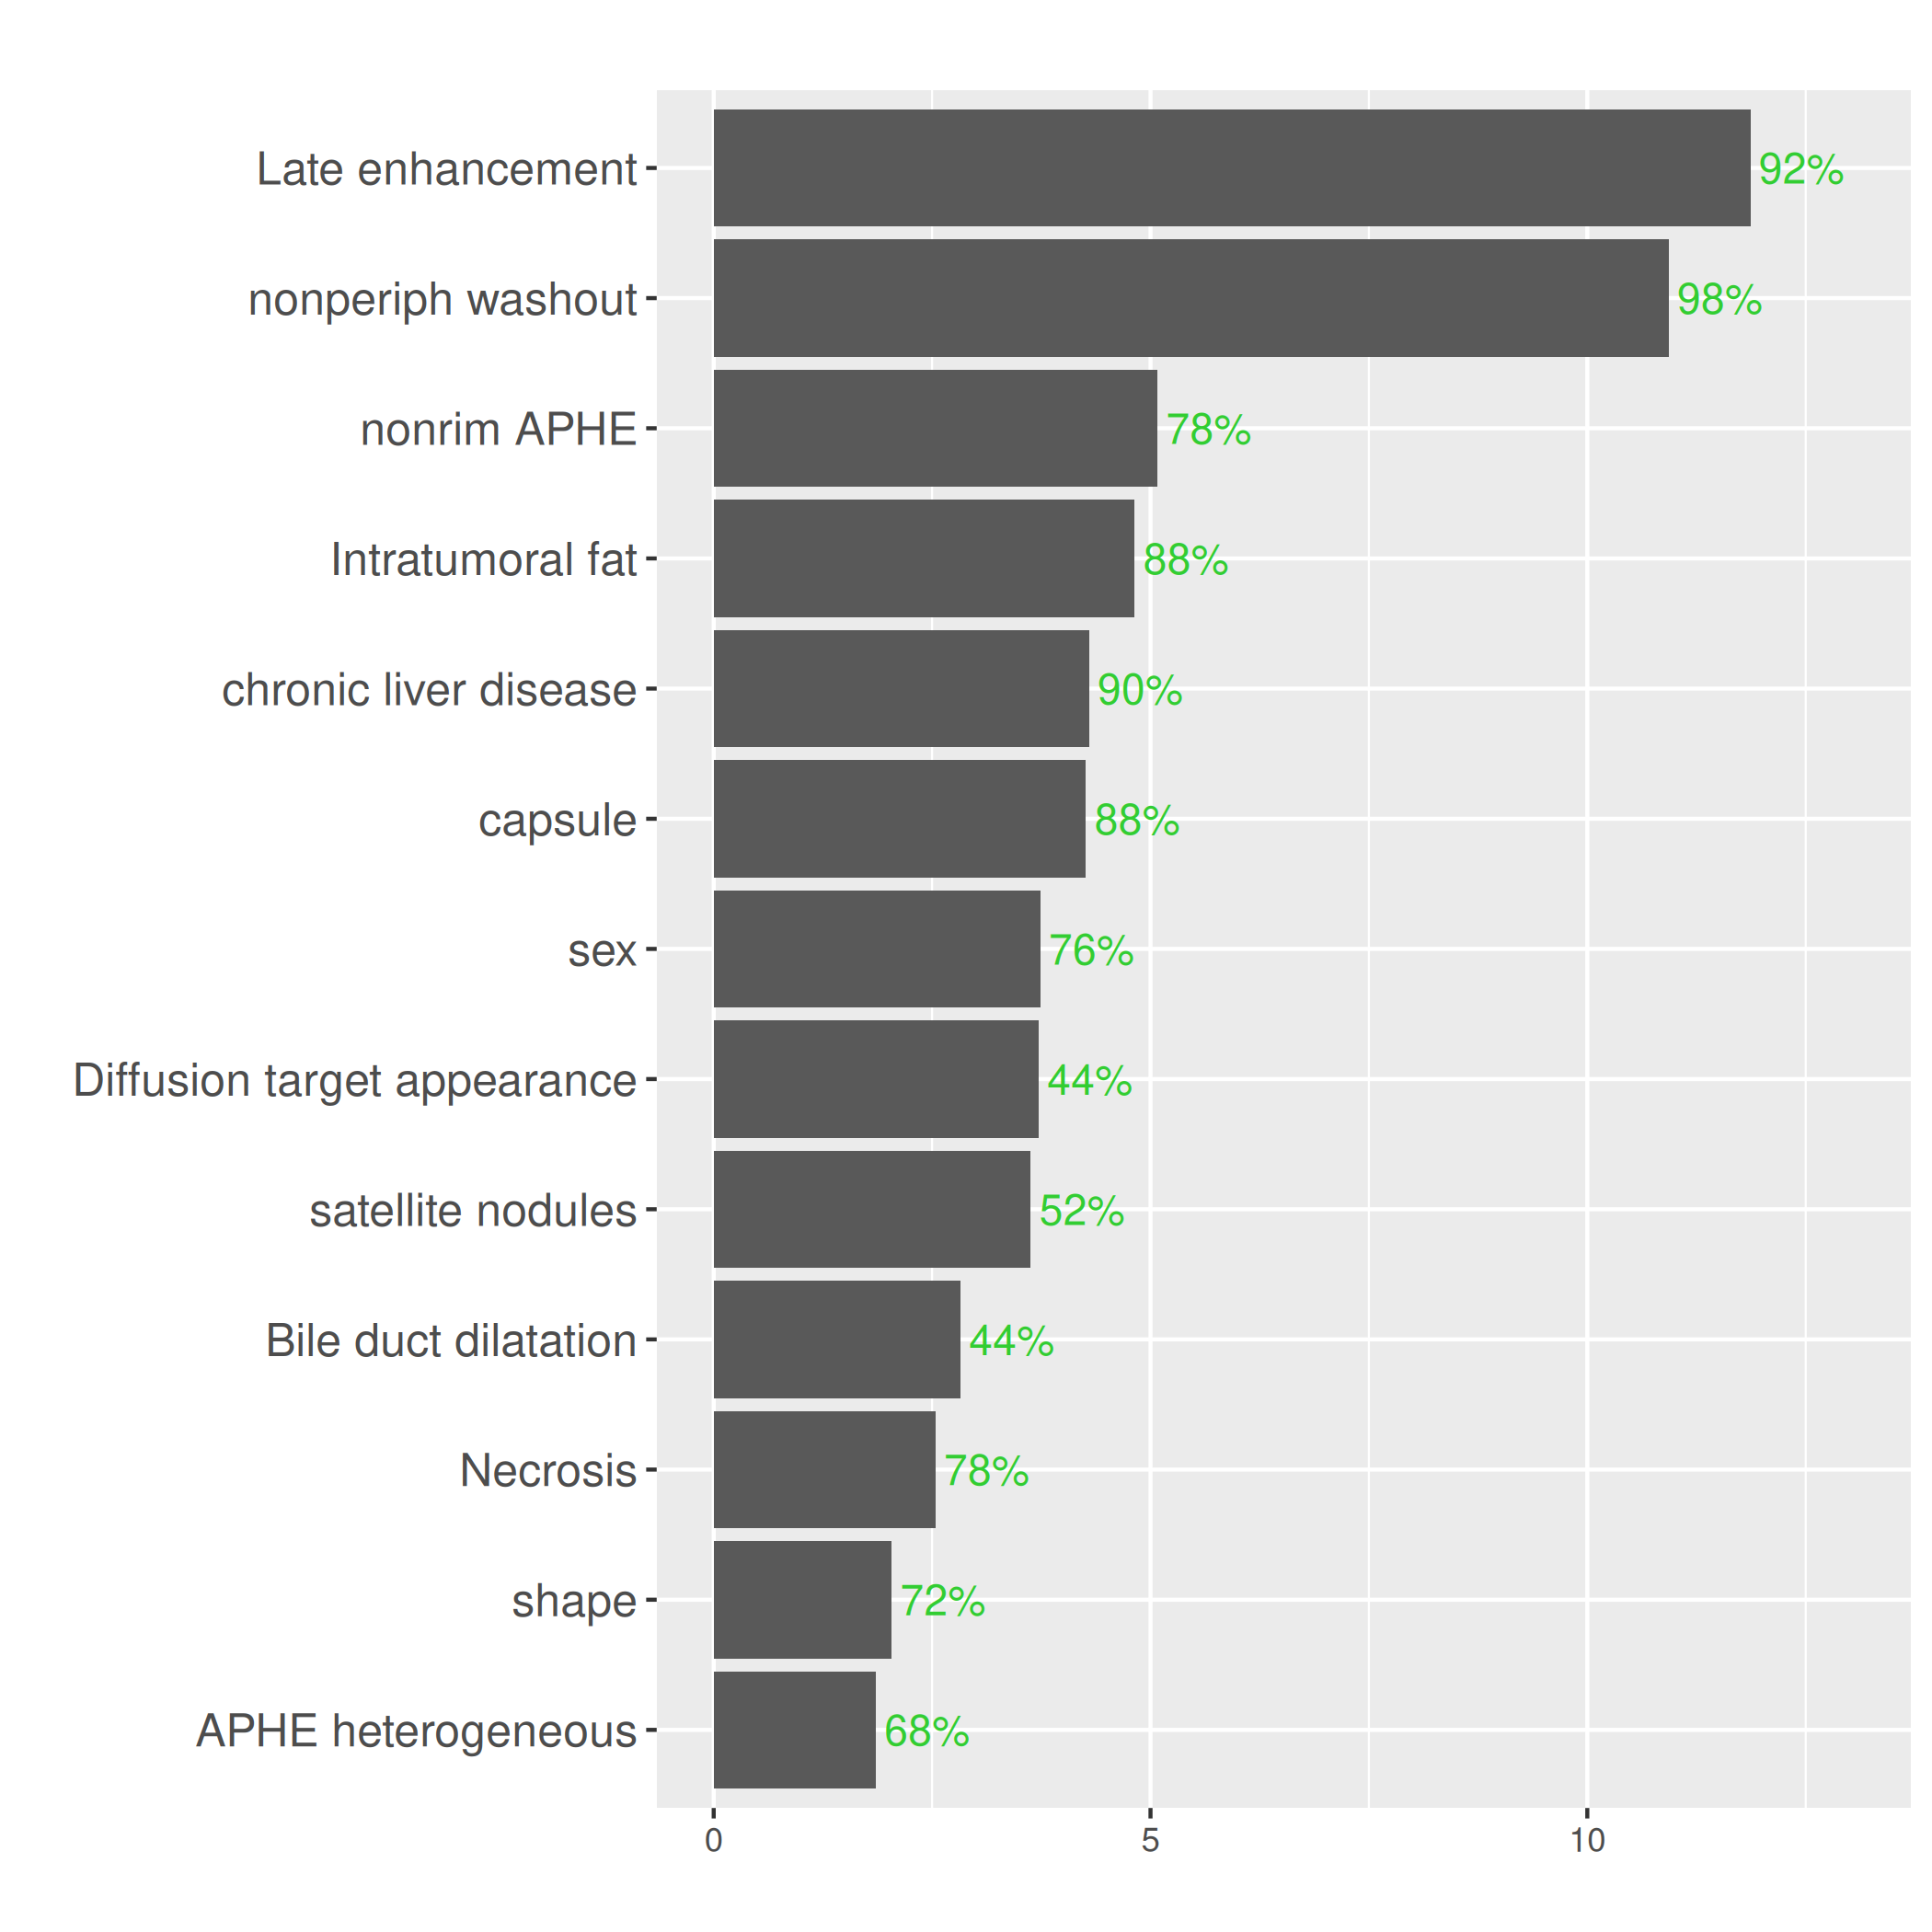
\includegraphics[scale = 0.38]{images/barplot_final.png}
%         \caption{Feature importance with lasso (in green percentage of runs with non null coefficient)}
%     \end{figure}
% \end{frame}


% \begin{frame}
%     \section{Retrospective Analysis}
% \end{frame}

% \begin{frame}
%     \frametitle{Personal learnings}
%     Direct impact: continuing in thesis (increase in motivation for research activities)\\[10 pt]
%     Soft skills in machine learning: becoming more critical vs results, searching for other data whenever possible\\[10 pt]
%     Being part of a team in a scientific context (not only 1 supervisor): importance of communication and reporting (even when no written documents)\\[10 pt]
%     Research in machine learning: an accessible world
% \end{frame}


% \begin{frame}
%     \frametitle{Conclusion}
%     A promising framework for the diagnosis of liver tumors\\[10 pt]
%     The simulation part of an article on the multiblock tensor model\\[10 pt]
%     Ethically positive impact (controllable deployment, a precise need, no replacement of human beings...)\\[20 pt]
%     \textbf{On a personal level}:\\[5 pt]
%     A good representation of a research work (and its challenges)\\[10 pt]
%     Supportive, available and calm supervision (even as deadlines approach)\\[10 pt]
%     Looking forward to continuing in this direction
% \end{frame}
\section*{Bibliography}
\begin{frame}
\sectionpage
\end{frame}


\begin{frame}[allowframebreaks] 
    \bibliographystyle{plain}
    \bibliography{bibliography.bib} 
    \end{frame}

    \section*{Annex}
\begin{frame}
\sectionpage
\end{frame}

\begin{frame}
    \frametitle{Lasso penalty in fitting algorithm}
    \begin{block}{Rewriting the penalty}
    \begin{align}
        \text{penalty} &\propto \sum\limits_{\ell,r} \left( \lVert \bm{\beta}_{\ell,r}^K \rVert_1 \lVert \bm{\beta}_{\ell,r}^J \rVert_1 \right)\\
        &= \sum\limits_{\ell,r} \left( \left\lVert  \lVert\bm{\beta}_{\ell,r}^K \rVert_1  \bm{\beta}_{\ell,r}^J \right\rVert_1 \right)  = \sum\limits_{\ell,r} \left( \left\lVert  \lVert\bm{\beta}_{\ell,r}^J \rVert_1  \bm{\beta}_{\ell,r}^K \right\rVert_1  \right)
    \end{align}
\end{block}
    \onslide<2->{
        \begin{block}{Strategy}
     dilate $\bm{\beta}_{\ell,r}^J$ by $\lVert \bm{\beta}_{\ell,r}^K\rVert_1$ and $x_{j,k}^\ell$ by $\lVert \bm{\beta}_{\ell,r}^K\rVert_1^{-1}$, so
     \vspace{-7 pt}
    $$\mathbf{x}^T\bm{\beta} \leadsto  \sum\limits_{j,\ell,r} \left(\sum\limits_{k}  x_{j,k}^\ell(\beta_{\ell,r}^{K})_k \, \right)(\beta_{\ell,r}^{J})_j$$\\[-10 pt]
     does not change but 
     \vspace{-7 pt}
     $$\lVert \bm{\beta}^J \rVert_1 \leadsto\sum\limits_{\ell,r} \left( \lVert \bm{\beta}_{\ell,r}^K \rVert_1 \lVert \bm{\beta}_{\ell,r}^J \rVert_1 \right) $$
\end{block}
    }
\end{frame}

\begin{frame}
    \begin{block}{New optimization problem}
        After the dilations presented in the previous slide, we get:
        \begin{align}
        \tilde{x}_{\ell,r,j} &= \sum\limits_{k}x_{j,k}^\ell\lVert \bm{\beta}_{\ell,r}^K\rVert_1^{-1}\\
        \tilde{\beta}_{l,r,j}^J &= 
        (\beta_{\ell,r}^J)_j\lVert \bm{\beta}_{\ell,r}^K \rVert_1 
        \end{align}
        \phantom{a}\hspace{40 pt}So that\\[-20 pt]
        \begin{align}
        \mathbf{x}^T\bm{\beta} & \leadsto  \langle \, \tilde{\underline{\mathbf{X}}}\,|\, \tilde{\underline{\mathbf{B}}}^J \,\rangle \\
        \text{penalty} &= \lambda \lVert \tilde{\underline{\mathbf{B}}}\rVert_1
        \end{align}
    \end{block}
    \frametitle{Lasso penalty in fitting algorithm}
    \noindent Thus, it is possible to do standard logistic lasso regression with $\tilde{\underline{\mathbf{X}}}$ (unfolded) as features and $\lambda$ as penalty to find the coefficients $\tilde{\underline{\mathbf{B}}}^J$, which can be easily related to those of the vectors ($\bm{\beta}_{\ell,r}^J$).\\[5 pt]
    Everything works symetrically for mode $K$.
\end{frame}

\begin{frame}
    \frametitle{Stopping criterion}
    \begin{block}{Penalized likelihood}
    $$C=  \log(\mathcal{L}(\bm{\beta})) -\text{penalty}$$
    \end{block}
    Before the t-th optimization cycle, its value is $C^{t}$ and after this cycle it becomes $C^{t + 1}$.\\[5 pt]
    \begin{block}{Stopping criterion}
    $$ |C^{t + 1} - C^t| < \epsilon |C^t|$$
    \end{block}
    (typically $\epsilon = 10^{-4}$)
\end{frame}

\begin{frame}
    \frametitle{Data generation}
    \begin{block}{Theorem for data generation}
    For a given $\bm{\beta}$ to be reconstructed (pictograms).\\[5 pt]
    If the $(\mathbf{x}_i)_{i \in \llbracket 1, I\rrbracket}$ are generated with 2 multivariate normal laws of means $\bm{\mu}_0$ and $\bm{\mu}_1$ and common covariance matrix $\bm{\Sigma}$ such that:
    \begin{itemize}
        \item $\bm{\mu}_1 - \bm{\mu}_0$ colinear to $\bm{\beta}$\\[10 pt]
        \item One of the principal axis of $\bm{\Sigma}$ colinear to $\bm{\beta}$
    \end{itemize}
    \vspace{5 pt}
    Then $\bm{\beta}$ is the normal vector to the best separating hyperplane between the two classes (which is in this case the Bayes classifier.)
\end{block}
Separation of classes is linked with eigenvalues of $\bm{\Sigma}$ (to be compared with $\lVert\bm{\mu}_1 - \bm{\mu}_0 \rVert$).
\end{frame}

\begin{frame}
    \frametitle{Future work}
    Testing on other real datasets wether the performances on the simulated dataset can be replicated.\\[10 pt]
    Testing other penalizations (group lasso, elastic net).\\[10 pt]
    Extending the multiblock approach to other classical machine learning algorithms (other GLMs, SVM etc...). Comparing it to CNN.\\[10 pt]
    Improving the optimization, by using coordinate descent (as done in glmnet \cite{glmnet} in R).
\end{frame}
\end{document}